\documentclass[11pt]{article}
\usepackage[T1]{fontenc}

% Set page size and margins
% Replace `letterpaper' with`a4paper' for UK/EU standard size
\usepackage[a4paper,top=2cm,bottom=2cm,left=3cm,right=3cm,marginparwidth=1.75cm]{geometry}

% Useful packages
\usepackage{amsmath}
\usepackage{graphicx}
\usepackage{amsfonts}
\usepackage{fancyhdr}
\setlength{\headheight}{15pt}
\pagestyle{fancy}

\usepackage{hyperref}
\hypersetup{
    colorlinks,
    citecolor=black,
    filecolor=black,
    linkcolor=black,
    urlcolor=black
}

\usepackage{glossaries}
\usepackage{subfigure}

\makenoidxglossaries


\loadglsentries{lexique}


\usepackage[table,xcdraw]{xcolor}
\usepackage{eso-pic}
\usepackage{tikz}
\usetikzlibrary{shapes,arrows,positioning}
\usepackage{float}
\usepackage{textcomp}
\usepackage{soul}
\usepackage{listings}
\newcommand{\hilight}{\makebox[0pt][s]{\color{green!50}\rule[-3.6pt]{1.0\linewidth}{12pt}}}

\usepackage{tikz}
\usepackage{listofitems} % for \readlist to create arrays


\tikzstyle{mynode}=[thick,draw=blue,fill=blue!20,circle,minimum size=22]


\definecolor{mygray}{rgb}{0.5,0.5,0.5}
\lstdefinestyle{command}{
  backgroundcolor=\color{white},
  basicstyle=\ttfamily\color{black},
  keywordstyle=\color{blue},
  commentstyle=\color{mygray},
  stringstyle=\color{red},
  showstringspaces=false,
  upquote=true,
  morekeywords={sudo, ls, cd, mv, cp, rm, mkdir, chmod, chown, grep, find},
  captionpos=b,
  frame=single,
  numbers=left,
  numberstyle=\tiny\color{mygray},
  breaklines=true,
  breakatwhitespace=true,
  tabsize=2,
  keepspaces=true,
  caption={Linux Command},
  label=command,
}
\lstdefinestyle{bashstyle}{
  backgroundcolor=\color{white},
  basicstyle=\ttfamily\color{black},
  keywordstyle=\color{blue},
  commentstyle=\color{mygray},
  stringstyle=\color{red},
  showstringspaces=false,
  upquote=true,
  morekeywords={sudo, ls, cd, mv, cp, rm, mkdir, chmod, chown, grep, find},
  captionpos=b,
  frame=single,
  numbers=left,
  numberstyle=\tiny\color{mygray},
  breaklines=true,
  breakatwhitespace=true,
  tabsize=2,
  keepspaces=true,
  caption={Script bash},
  label=command,
}

\lstdefinestyle{cstyle}{
    language=C,
    basicstyle=\ttfamily,
    keywordstyle=\color{blue},
    commentstyle=\color{green!40!black},
    stringstyle=\color{red},
    identifierstyle=\color{black},
    captionpos=b,
    numbers=left,
    numberstyle=\tiny\color{gray},
    frame=single,
    breaklines=true,
    showstringspaces=false,
    tabsize=4,
    morekeywords={int, char, void, if, else, while, for, return, typedef, struct, include},
    columns=flexible
}

\lstdefinestyle{makefilestyle}{
    language=make,
    basicstyle=\ttfamily,
    keywordstyle=\color{blue},
    commentstyle=\color{green!40!black},
    captionpos=b,
    stringstyle=\color{red},
    identifierstyle=\color{black},
    numbers=left,
    numberstyle=\tiny\color{gray},
    frame=single,
    breaklines=true,
    showstringspaces=false,
    tabsize=4,
    morekeywords={ifeq, endif, else, ifdef, ifndef, define, endef, export, unexport, obj},
    columns=flexible
}
\lstdefinestyle{config}{
    language=make,
    basicstyle=\ttfamily,
    keywordstyle=\color{blue},
    commentstyle=\color{green!40!black},
    captionpos=b,
    stringstyle=\color{red},
    identifierstyle=\color{black},
    numbers=left,
    numberstyle=\tiny\color{gray},
    frame=single,
    breaklines=true,
    showstringspaces=false,
    tabsize=4,
    morekeywords={ifeq, endif, else, ifdef, ifndef, define, endef, export, unexport, obj},
    columns=flexible
}

\bibliographystyle{plain} % We choose the "plain" reference style

\renewcommand{\epsilon}{\varepsilon} 
\renewcommand{\phi}{\varphi} 
\title{Final Year Project Report\vspace{10pt}\\
**************************************************\\
Multi Agent Scene Exploration and Mapping \\
for Continuous Digital Twin Creation\vspace{10pt}\\
**************************************************}
\author{BELPOIS Vincent \\ Under the supervision of Dr. Ivan \textsc{Mutis}}

\begin{document}

\date{2024}
\maketitle
\thispagestyle{empty}

\vspace{10mm}

    \begin{center}
    
\includegraphics[width = 6cm]{Images/logo_ensma.png}
    \end{center}
    \vspace{2cm}
    \begin{center}
        
\includegraphics[width = 8cm]{Images/IIT_Logo_stack_186_blk.png}
    \end{center}
    \vspace{1cm}
    \begin{center}
        
\includegraphics[width = 6cm]{Images/logo_iconsense_bloack_text.png}
    \end{center}
    \newpage
    \thispagestyle{empty}
    \mbox{}
    
    

    
    \AddToShipoutPictureBG{%
    \put(15,7){
\includegraphics[scale = 0.02]{Images/logo_ensma.png}}
    \put(480,10){
\includegraphics[width = 100pt]{Images/IIT_Logo_stack_186_blk.png}}
    \put(400,14.9){
\includegraphics[width = 75pt]{Images/logo_iconsense_bloack_text.png}}
    }



    \newpage
    \section*{Acknowledgments}

        Acknowledgments.
        
    \newpage
    \thispagestyle{empty}
    \mbox{}
    \newpage
    \thispagestyle{empty}
    {\small \tableofcontents}

    \newpage
    \thispagestyle{empty}
    \mbox{}
    \newpage
    
    \section{Introduction}
    
    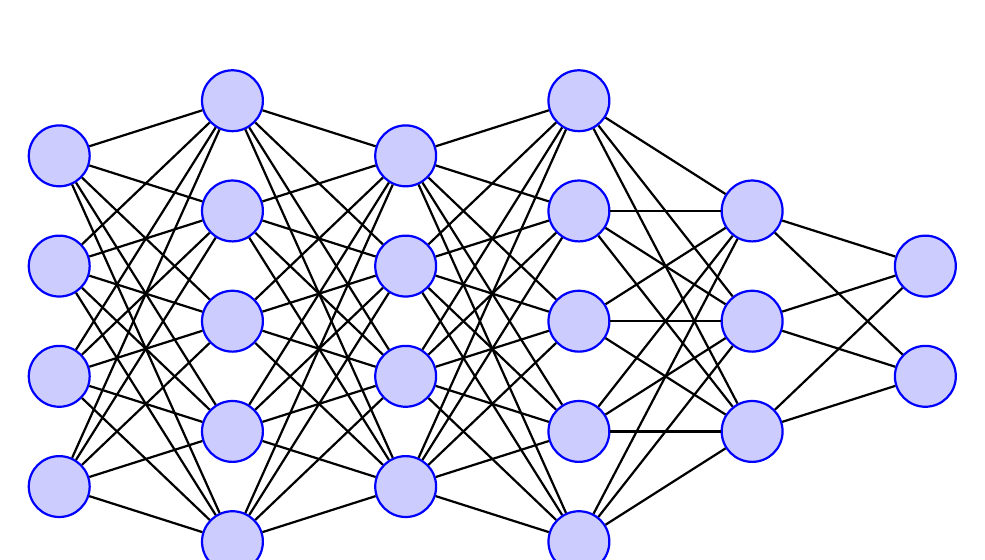
\begin{tikzpicture}[x=2.2cm,y=1.4cm]
        \readlist\Nnod{4,5,4,5,3,2} % number of nodes per layer
        % \Nnodlen = length of \Nnod (i.e. total number of layers)
        % \Nnod[1] = element (number of nodes) at index 1
        \foreachitem \N \in \Nnod{ % loop over layers
          % \N     = current element in this iteration (i.e. number of nodes for this layer)
          % \Ncnt  = index of current layer in this iteration
          \foreach \i [evaluate={\x=\Ncnt; \y=\N/2-\i+0.5; \prev=int(\Ncnt-1);}] in {1,...,\N}{ % loop over nodes
            \node[mynode] (N\Ncnt-\i) at (\x,\y) {};
            \ifnum\Ncnt>1 % connect to previous layer
              \foreach \j in {1,...,\Nnod[\prev]}{ % loop over nodes in previous layer
                \draw[thick] (N\prev-\j) -- (N\Ncnt-\i); % connect arrows directly
              }
            \fi % else: nothing to connect first layer
          }
        }
      \end{tikzpicture}

        $$
        \int_\alpha^\beta f(x) dx
        $$
        \cite{xu2022fast}


    \newpage
    
    \section[Setting up the physical agents]{Setting up the physical agents}
    \label{section:big title}%label to reference section

            Three platforms were used in this project: a six-wheeled platform, a quadcopter, and a quadruped platform. Each platform was chosen for its specific characteristics, with the goal of having a multi-agent system that could explore and map a scene. The six-wheeled platform was chosen for its stability and ability to carry heavy loads. The quadcopter was chosen for its ability to fly and provide a bird's-eye view of the scene. The quadruped platform was chosen for its ability to climb stairs and navigate bumpy terrain.
    
        \subsection{Six wheeled platform setup}

            The six-wheeled platform was chosen for its stability and its ability to carry heavy loads. The intent was to have it carry a robotic arm for other projects. Some previous work had already been done on the platform but was apparently unsuccessful. These earlier attempts had left the platform in a partially modified state, requiring a comprehensive reassessment and redesign of both the mechanical and electrical systems. Despite these setbacks, the robust chassis of the six-wheeled platform still presented an excellent foundation for our project, offering the potential for further development.

            \subsubsection{Mechanical modifications}
            As it arrived, the six-wheeled platform only consisted of a stainless steel chassis, six DC motors, and wheels. The platform required several mechanical modifications to accommodate the necessary components for autonomous operation. Specifically, it needed a mount for a LIDAR sensor and an embedded computer on its top surface (see Figure \ref{fig:LIDAR_mount}). Additionally, a mounting solution for the motor drivers inside the chassis was essential (see Figure \ref{fig:motor_driver_mount}). These modifications were designed and implemented to ensure proper integration of all components while maintaining the structural integrity of the platform (see Figure \ref{fig:full_cad_model}).

            \begin{figure}[htbp]
                \centering
                LIDAR MOUNT CAD
                %\includegraphics[width=0.8\textwidth]{images/lidar_mount_cad.png}
                \caption{CAD model of the LIDAR sensor and embedded computer mount}
                \label{fig:LIDAR_mount}
            \end{figure}
            
            \begin{figure}[htbp]
                \centering
                MOTOR DRIVER MOUNT CAD
                %\includegraphics[width=0.8\textwidth]{images/motor_driver_mount_cad.png}
                \caption{CAD model of the motor driver mounting solution}
                \label{fig:motor_driver_mount}
            \end{figure}
            
            \begin{figure}[htbp]
                \centering
                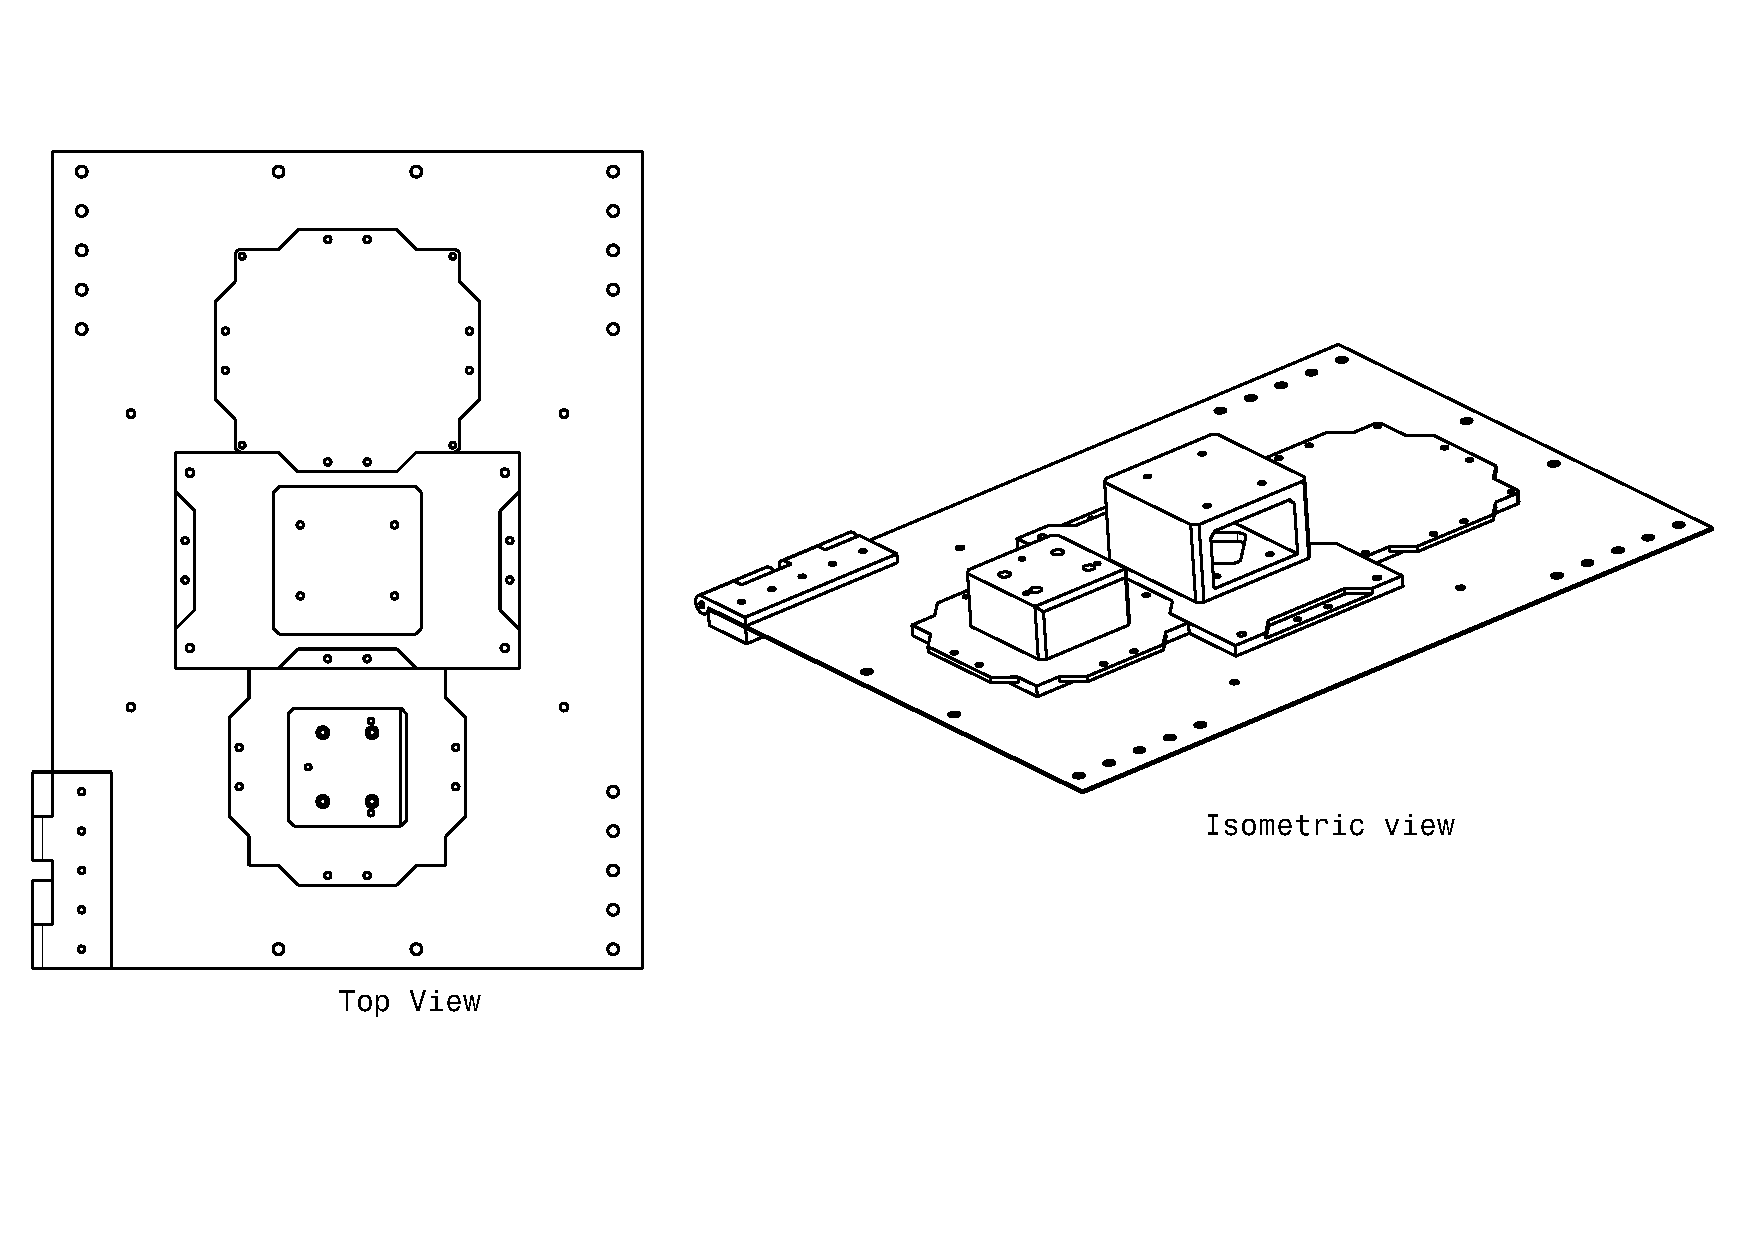
\includegraphics[width=0.8\textwidth]{Images/ViewRoverV1.pdf}
                \caption{CAD model of the modified six-wheeled platform's top}
                \label{fig:full_cad_model}
            \end{figure}

            \subsubsection{Electronics architecture}
                The essential electronic components needed to get the platform running were mainly DC motor drivers to drive the motors, a LIDAR sensor and an embedded computer.
                
                Difficulties were encountered when trying to use the drivers someone else tried before hand as they were underpowered : at stall, the motors required around 5 amps, as measured with a bench top power supply, and the drivers I was trying to use were only capable of delivering 2 amps per channel or a total of 4 amps when combining outputs. The drivers in question were the based on the LN298N which were in terms replaced by the 7A dual motor drivers from DFRobot. A physical comparison can be seen in \ref{fig:drivers_comparison}
                
                Difficulties were encountered when trying to use the drivers someone else tried before hand as they were underpowered : at stall, the motors required around 5 amps, as measured with a bench top power supply, and the drivers I was trying to use were only capable of delivering 2 amps per channel or a total of 4 amps when combining outputs. The drivers in question were the L298N H-bridge motor drivers, which were ultimately replaced by the DFRobot 7A Dual DC Motor Driver. The L298N drivers, while popular for smaller projects, proved inadequate for the power requirements of our six-wheeled platform. In contrast, the DFRobot 7A Dual DC Motor Driver offer a continuous current output of 7A per channel, more than sufficient for our needs. This upgrade significantly improved the platform's performance, allowing for smoother operation and better handling of the motor's power demands. A physical comparison of these drivers can be seen in Figure.\ref{fig:drivers_comparison}.

                
                \begin{figure}[h]
                    \centering
                    %INSERT (a) (b) PICTURE OF BOTH DRIVERS
                    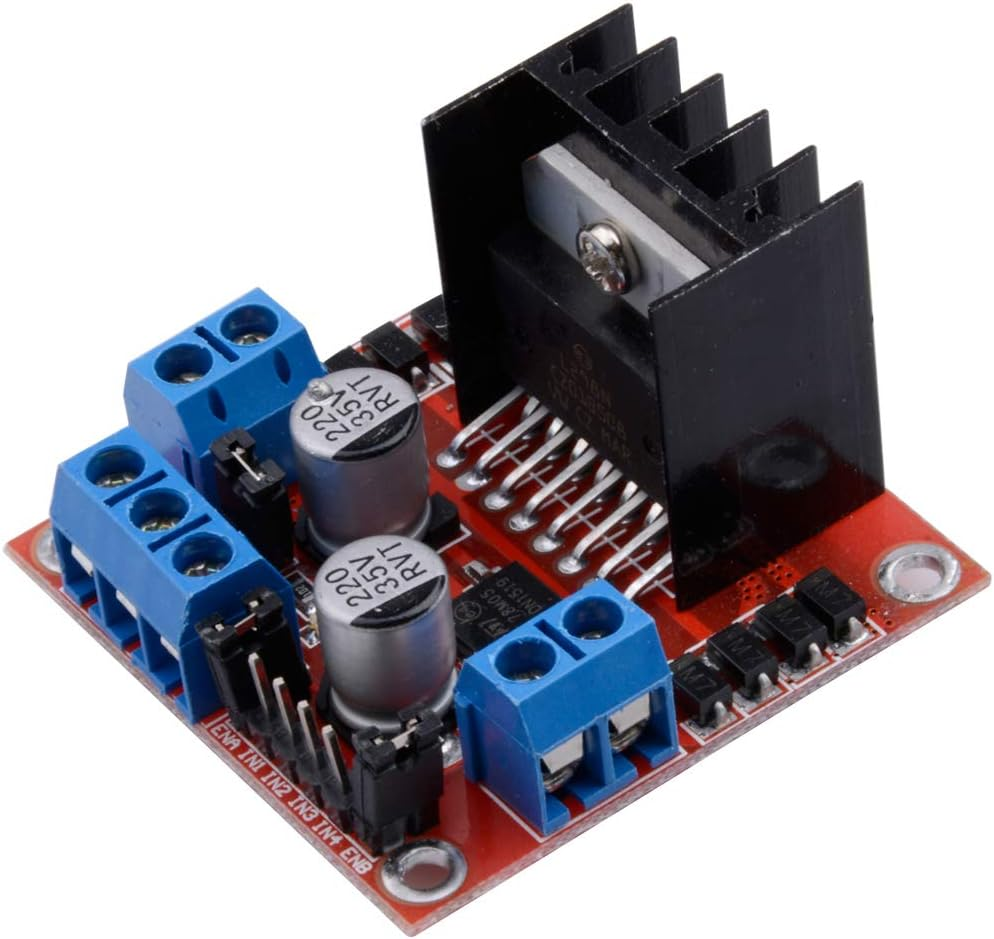
\includegraphics[width=0.3\textwidth]{Images/olddrivers.jpg}
                    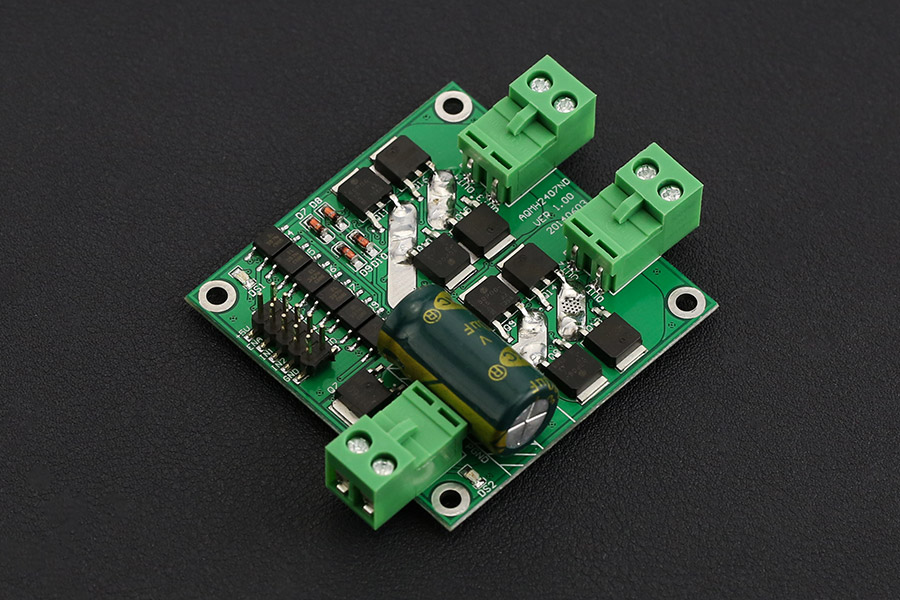
\includegraphics[width=0.4\textwidth]{Images/newdrivers.jpg}
                    \caption{L298N (a) and DFRobot 7A dual DC Motor Driver (b)}
                    \label{fig:drivers_comparison}
                \end{figure}

                The three motor drivers were connected to a microcontroller. The connection can be seen in \ref{fig:driver_to_pico}.
                I chose to use a Raspberry Pi Pico microcontroller for its many outputs, totaling 26 general purpose input outputs (GPIO). Each driver required 6 control signals or 3 per motor: two signals are used to control the direction of the motor according to Table \ref{tab:motor_control}, while the third signal's duty cycle determines the speed.

                A radio control (RC) receiver was also connected to interrupt capable GPIOs of the microcontroller to be able to control the platform manually. Three channels of the RC receiver were used to control the speed, the direction and the mode of the platform. The mode refers to whether or not the platform is in manual control or in autonomous mode and is connected to channel 5 of the radio which has a two way switch.

                Finally, the pico is connected to an Nvidia Jetson Orin single board computer (SBC) via USB. This connection is used both to reprogram the pico, as well as to send speed and direction commands to each motor via a serial communication. 

                Not including the power distribution and regulation system, \ref{fig:overall_electical_system} shows the electrical connections of these components on the modified six-wheeled platform.


                \begin{table}[h!]
                    \centering
                    \begin{tabular}{|c|c|c|c|}
                    \hline
                    IN1 & IN2 & ENA/ENB & Motor1/2 Behavior \\ \hline
                    0   & 0   & x       & Stop (brake)      \\ \hline
                    1   & 1   & x       & Vacant            \\ \hline
                    1   & 0   & 1       & Forward 100\%     \\ \hline
                    0   & 1   & 1       & Reverse 100\%     \\ \hline
                    1   & 0   & PWM     & Forward at PWM speed \\ \hline
                    0   & 1   & PWM     & Reverse at PWM speed \\ \hline
                    \end{tabular}
                    \caption{Motor Control Table}
                    \label{tab:motor_control}
                \end{table}

                %! Add a reference to this figure !!
                \begin{figure}[H]
                    \centering
                    %OVERALL ELECTRICAL SYSTEM (excluding power)
                    
                    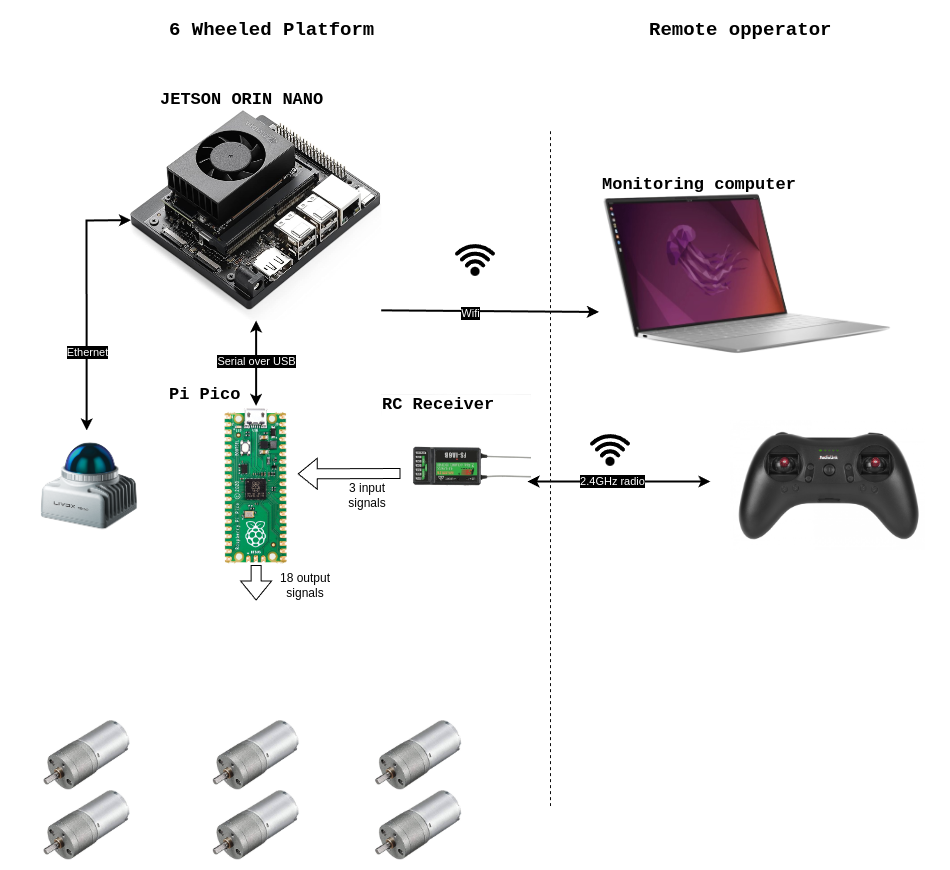
\includegraphics[width=0.8\textwidth]{Images/PFE-Page-2.drawio.png}
                    \caption{Overall electrical system, excluding power distribution and regulation}
                    \label{fig:overall_electical_system}
                \end{figure}


                
                
                \begin{figure}[h]
                    \centering
                    Driver to PICO connection diagram
                    \label{fig:driver_to_pico}
                \end{figure}

            
            
            \subsubsection{Software architecture}

            %How the software on the jetson communicates with the microcontroller and how it communicates with the LIDAR. The choice of the odometry algorithm will be explain in another section (master, comparison of multiple algo)

            The robot operation system (ROS) was chosen as the software framework for the platform running on the Jetson Orin embedded computer. Specifically, ROS2 Humble Hawksbill was selected due to its extensive package availability and compatibility with the Jetson Orin's hardware. Indeed, I was made aware of the strugles of another researcher running a ROS based robot on an Nvidia Jetson Nano and how Ubuntu, and ROS version mismatch may bring problems. 
            
            This version of ROS2 provides a robust and flexible framework for developing and integrating various components of the platform, including sensor processing, navigation, and control. For real-time critical tasks such as motor control and RC radio interrupts, the Raspberry Pi Pico microcontroller was utilized, leveraging its ability to handle low-level, time-sensitive operations. The microcontroller's firmware was developed from the ground up by myself, guaranteeing reliable execution of motor control and interrupt handling tasks. By combining the strengths of ROS2 on the Jetson Orin with the real-time capabilities of the Raspberry Pi Pico, the platform achieves a robust and efficient software architecture that enables seamless integration of autonomous navigation, sensor processing, and manual control.

            %! Add a reference to this figure !!
            \begin{figure}[H]
                \centering
                %Software stack, from jetpack to ros2 to the nodes to the microcontroller
                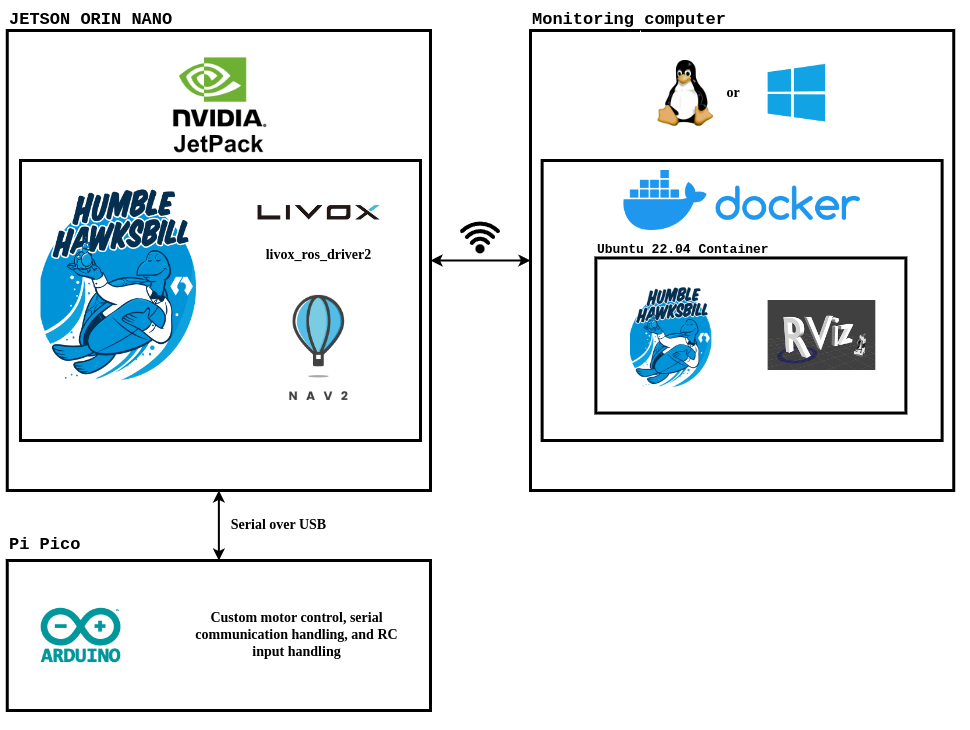
\includegraphics[width=0.8\textwidth]{Images/Software architecture rover.drawio.png}
                \caption{Software architecture}
                \label{fig:SW_architecture}
            \end{figure}


            \subsubsection{ROS 2 setup}
            
            % What nodes did I create, explain the setup with nav2 working.
            

            \subsubsection{Issues encountered}
                
            %Explain the state reached (nav2 navigation kinda working) and why the other platform was created

            The 6-wheeled rover, with its stainless steel frame and weak DC motors lacking encoders, was not the most suitable platform for the task of autonomous navigation. The lack of encoders on the motors made odometry calculations based on the LIDAR and inertial measurement unit unreliable. An attempt was made to do closed-loop control with the aforementioned odometry, but the noise and the lack of per-wheel odometry made it impossible to have a stable and reliable control. I then decided to create a new platform using closed-loop stepper motors, also called servos. Their closed-loop control and high torque at low speed would make them ideal for slow movements, thereby making the task of autonomous navigation feasible.

            %! Add a reference to this figure !!
            \begin{figure}[h!]
                \centering 
                \subfigure[Version 1 of the rover]{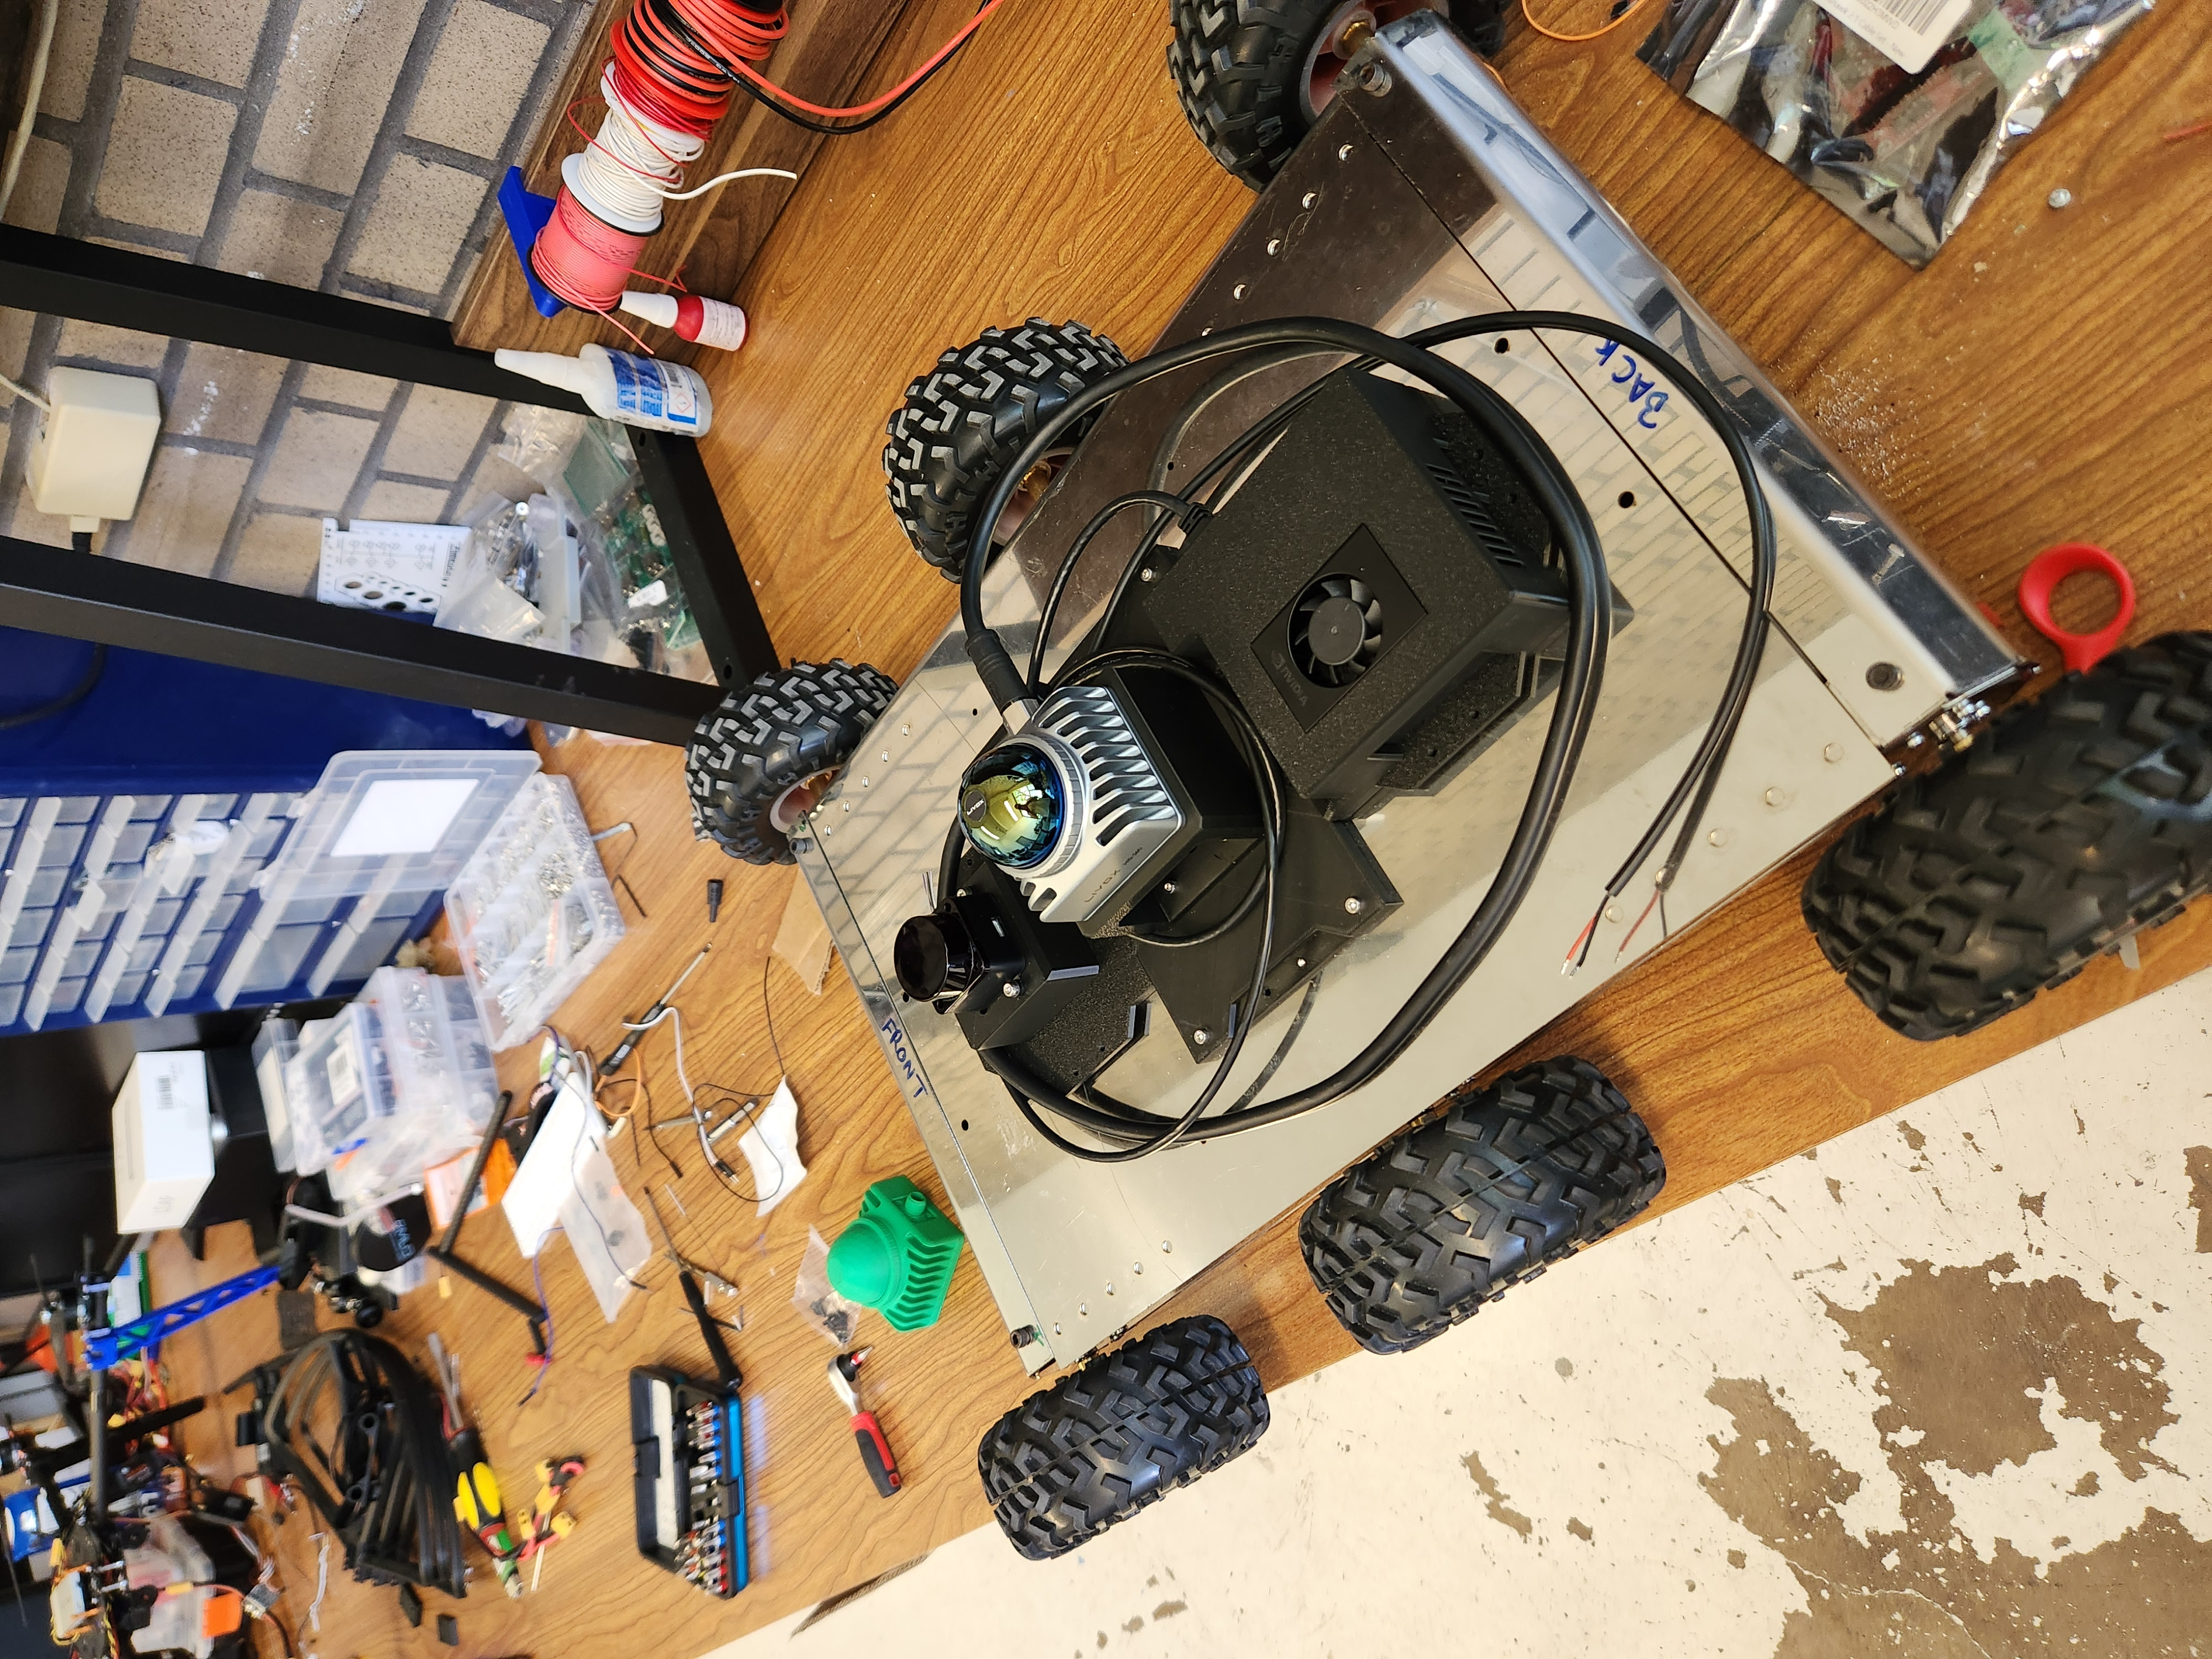
\includegraphics[width=0.4\textwidth, angle=270]{Images/roverv1closed.jpg}}
                \subfigure[Version 2 of the rover]{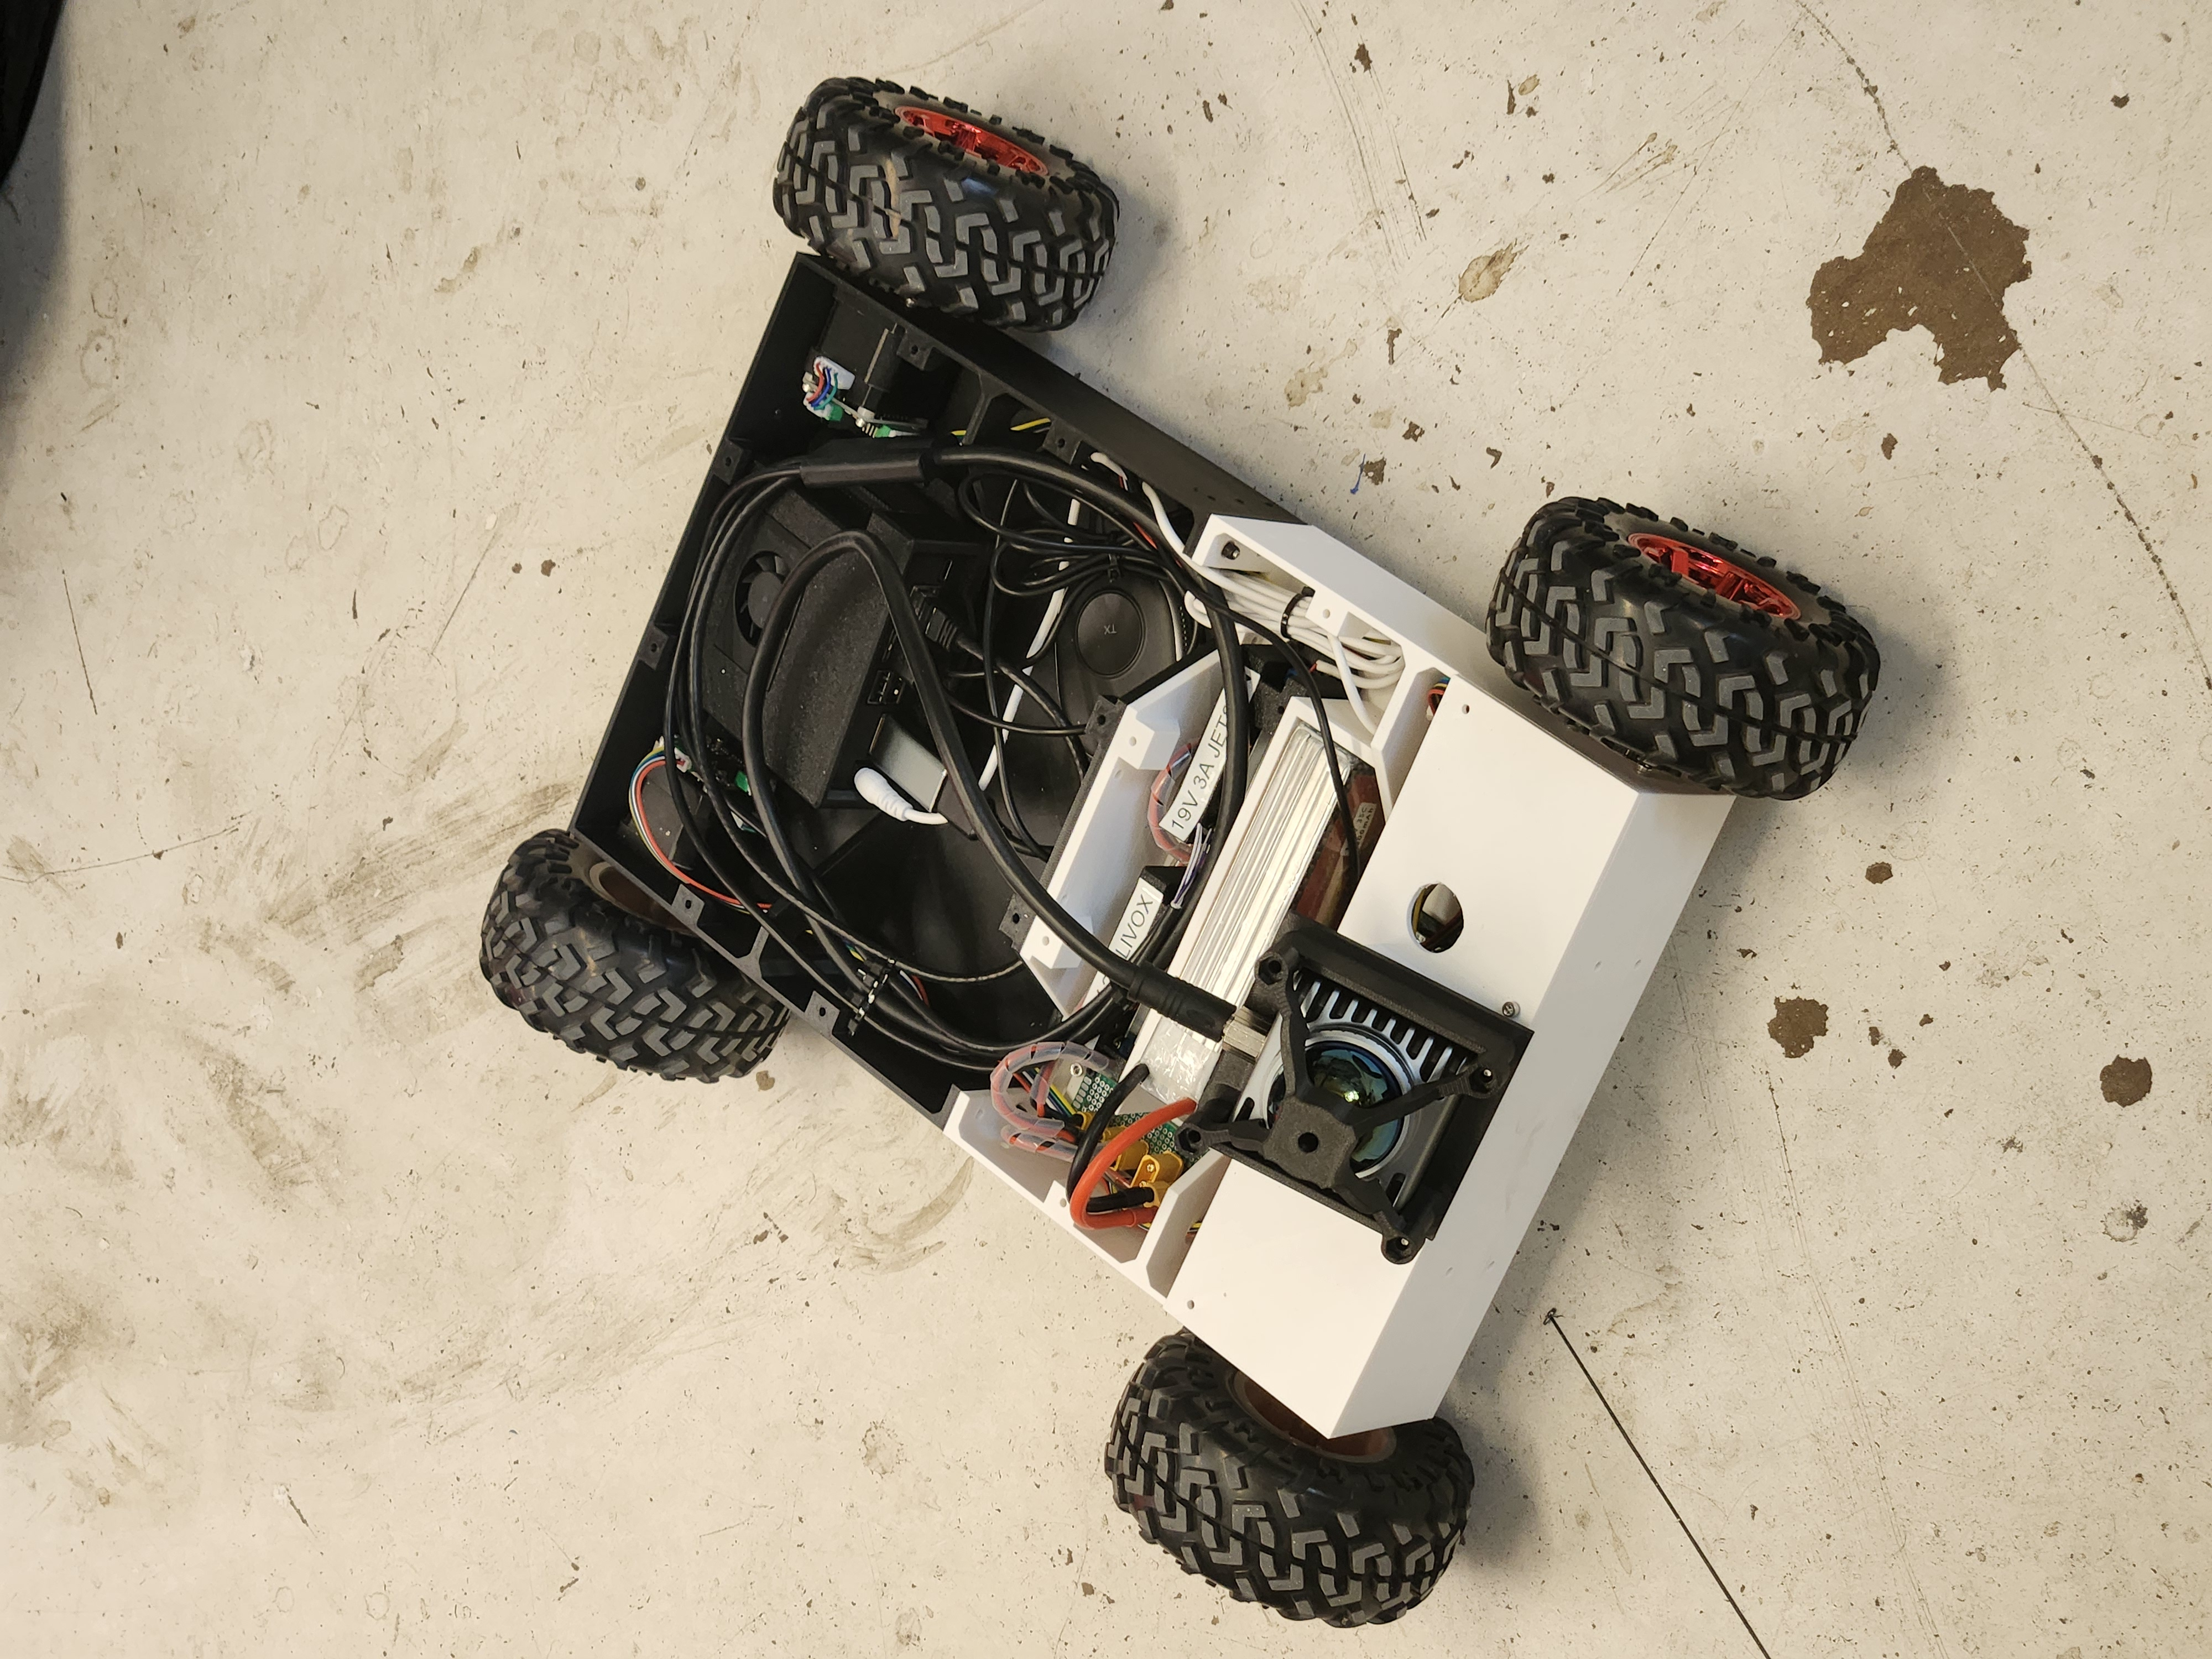
\includegraphics[width=0.4\textwidth, angle=270]{Images/roverv2openened.jpg}}       
                \caption{Rover version 1 and 2}
            \end{figure}


            %Explain how the chassis was designed to fit the new closed loop, motors

        \subsection{Quadcopter setup}
                
                % Explain the platform's starting point and the goal
                % Explain the different drones that were at my disposal and which one was selected for our application (the one that could easel;y carry the LIDAR, jetson while not being too big)

                One of the agents in our multi-agent system is a quadcopter, chosen for its ability to provide aerial perspective and navigate in three-dimensional space. After evaluating several drone options available to us, we selected a model that struck an optimal balance between payload capacity and size. This drone was capable of easily carrying the Livox Mid-360 LIDAR sensor and the Nvidia Jetson Orin embedded computer, while still maintaining a compact form factor suitable for indoor and outdoor operations.

                The quadcopter platform required several modifications to integrate our specific sensor suite and computational hardware.

                \subsubsection{Mechanical modifications}

                    I designed and 3D printed new landing legs that fit on the arms of the quadcopter. Those landing legs were designed to increase the landing stability, which I noticed was a problem in the manual flight I performed, and to reduce the blindspots of the LIDAR which was to be placed on the center of the underside of the drone.

                    I also took the oportunity to redisgne the battery mounting mechanism which was bulky, heavy, and suitable to only one size of battery to one that is much simpler and uses velcro straps as can been seen in Figure \ref{fig:landing_legs}. This resulted in a saving of \color{red} XXX grams \color{black} and thus increased the flight time of the drone. 
                    

                    \begin{figure}[H]
                        \centering
                        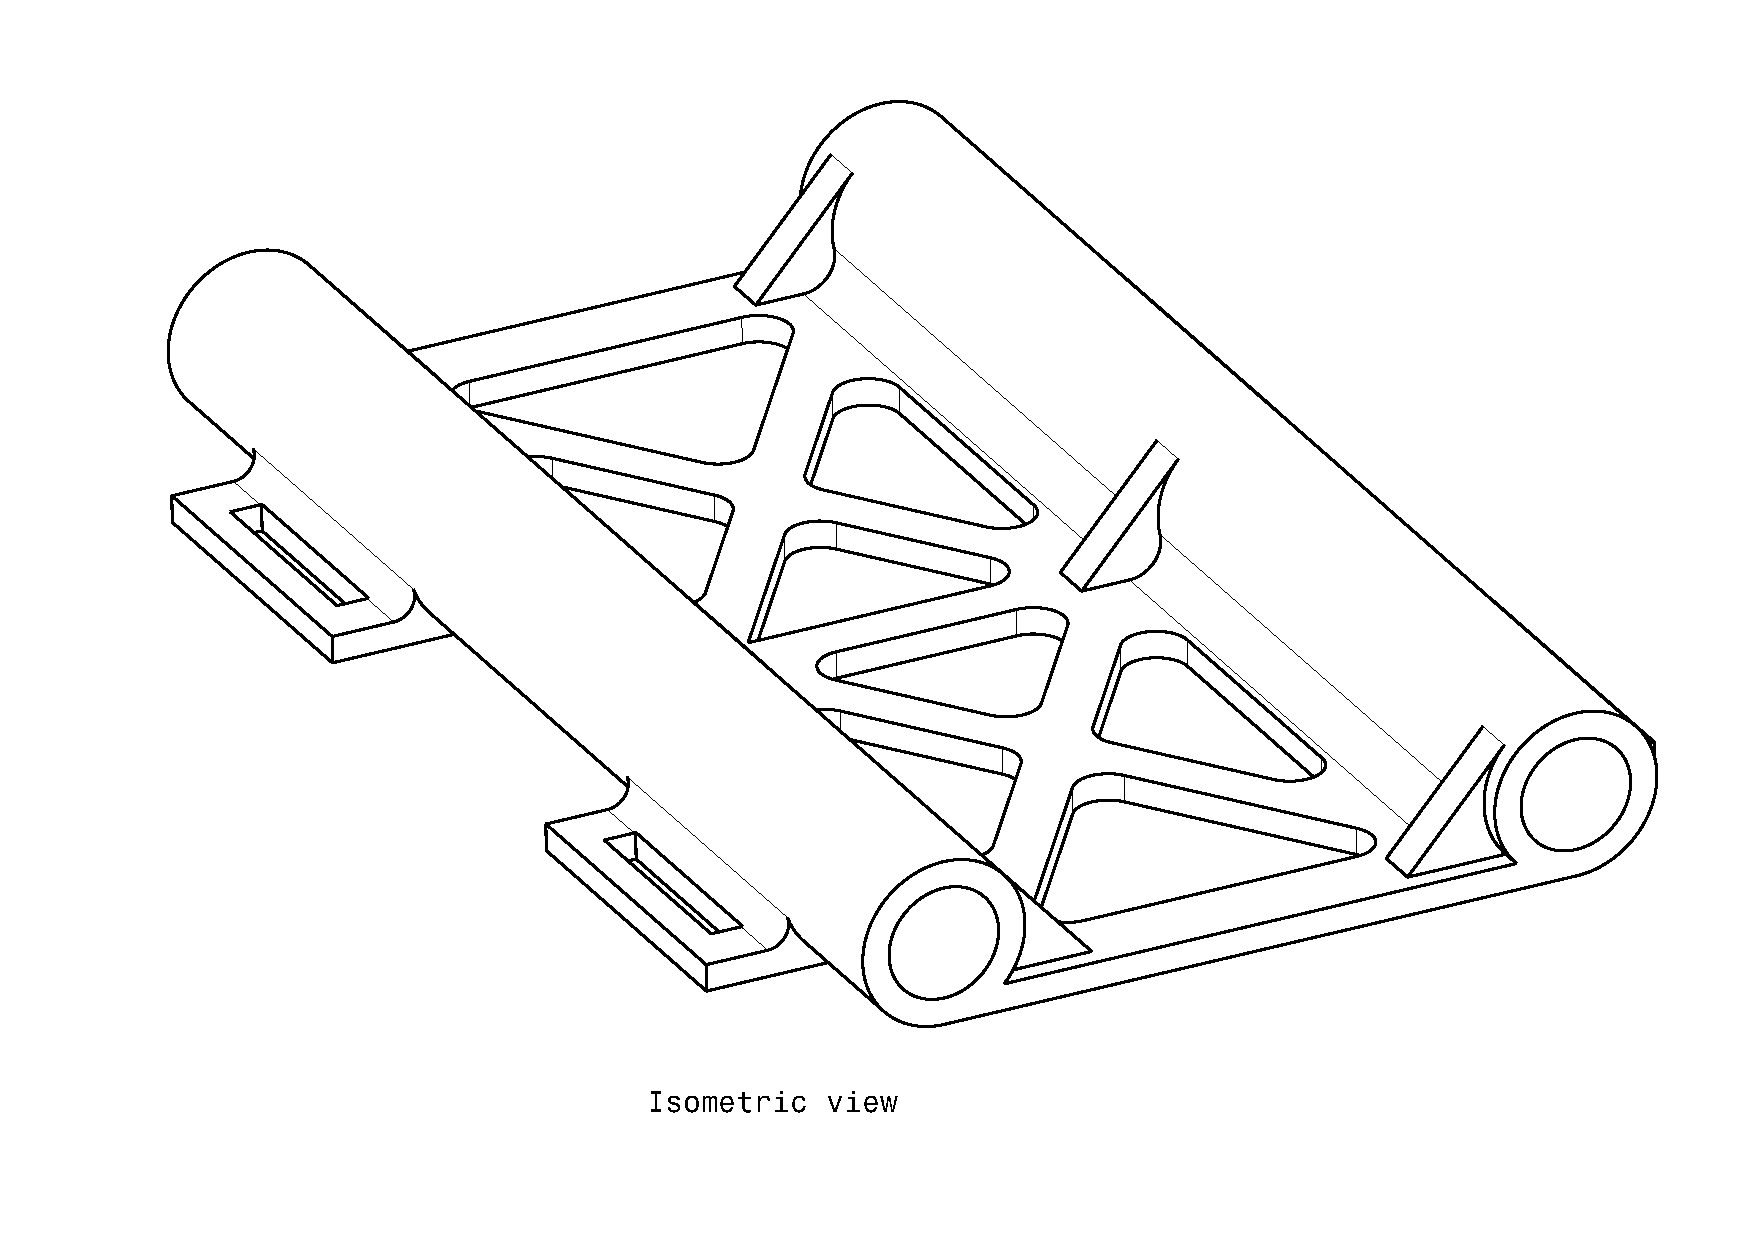
\includegraphics[width=0.6\textwidth]{Images/BatteryTrayDrawing.pdf}
                        \caption{New battery tray}
                        \label{fig:landing_legs}
                    \end{figure}    
                \subsubsection{Electronics architecture}
    
                    % Similarly to the rover, the jetson is still connected to the LIDAR via ethernet 
                    % The drone is controlled by a PLACEHOLDER_CONTROLLER, which is connected to the jetson via USB

                    To keep the architecture similar to the one used on the wheeled robot, the quadcopter was also equipped with an Nvidia Jetson Orin embedded computer and a Livox MID-360 LIDAR. The computer and the LIDAR get their power from the drone's battery, which is regulated to 19V and 12V respectively.

                \subsubsection{Software architecture and setup}
                    
                    % don't know what planner to use, something complicated or just a grid coverage planner
            
                \subsubsection{Issues encountered}
                
        \subsection{Quadruped platform setup}

            A gadruped was chosen as the third platform as it can navigate rough terrain and climb stairs. The platform chosen was the Unitree GO2, a quadruped robot with a 3D LIDAR and an embedded computer.

            \subsubsection{Compute backpack}

            Even though the Unitree GO2 has a LIDAR of it's own and an embeded computer based on the Rockchip RK3588S inside, we decided to add an aditional LIDAR on top of the platform and as such needed an aditional embedded computer.

            As is the case with the wheeled platform and the drone, we chose to use a Livox Mid-360 LIDAR and a Nvidia Jetson Orin embedded computer. Even though the quadruped already carries a 3D LIDAR, we chose to use a Mid-360 as the ladder produces around ten times more points per second (21600 points per second for the Unitree L1 LIDAR against the 200000 points per second of the MID-360).

            \begin{figure}[H]
                \centering
                \begin{minipage}{0.45\textwidth}
                    The compute backpack also provides access to a power port with a connector Amass XT-30 and a gigabit ethernet port on the robot that are usually covered by a plastic cover. Those ports are covered by the handle of the GO2 as can be seen in the figure \ref{fig:handle_cover}.
                \end{minipage}%
                \hfill
                \begin{minipage}{0.5\textwidth}
                    \centering
                    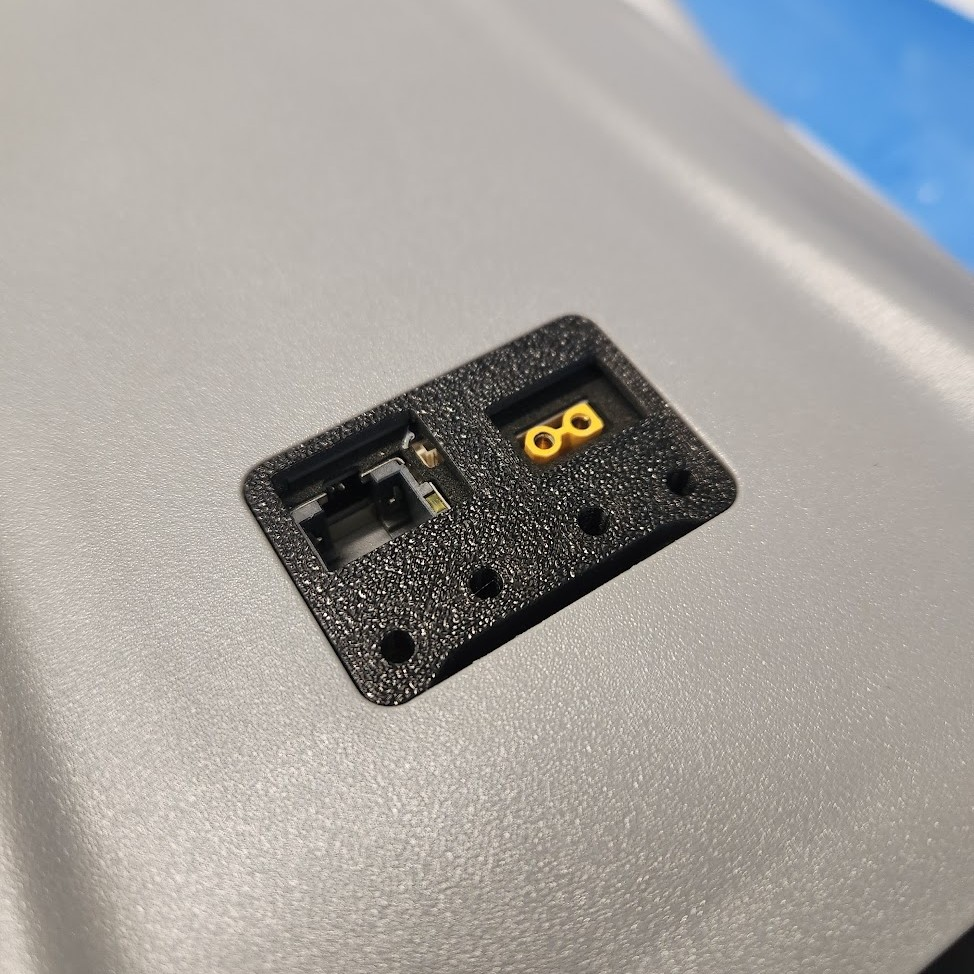
\includegraphics[width=0.75\textwidth]{Images/PortsWithCover.jpg}
                    \caption{Handle and covered connectors}
                    \label{fig:handle_cover}
                \end{minipage}
            \end{figure}
            To fit the Nvidia Jetson, the LIDAR, and the power regulators needed for both of them, the top part of the robot was scanned and a new top part was designed and 3D printed. The CAD model of top part and the scan can be seen in figure \ref{fig:scanner_and_cad}. This holds the LIDAR on the back of the robot to be sure to cover the grounds during the scanning process. The angle was determined as to not have any of the robot itself in the field of view of the LIDAR.

            \begin{figure}[H]
                \centering
                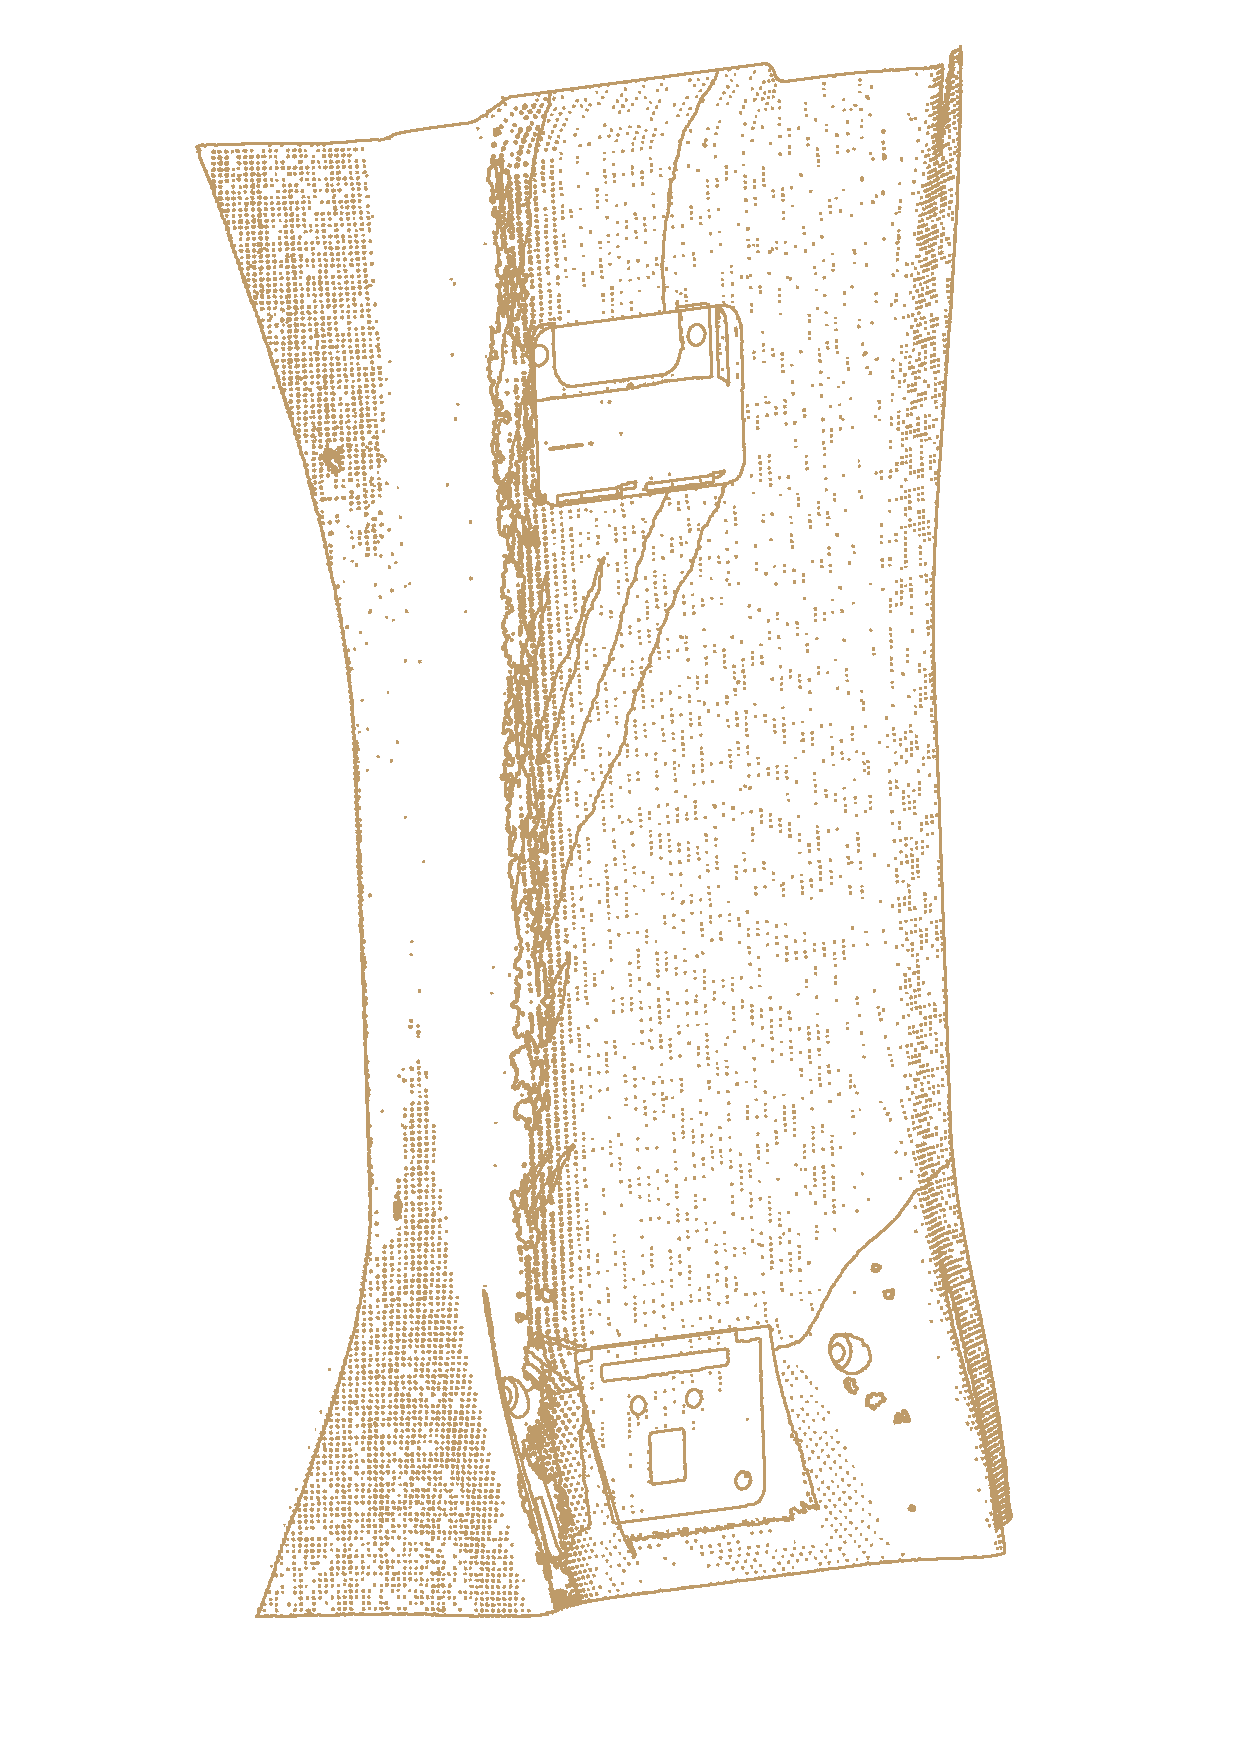
\includegraphics[width=0.3\textwidth]{Images/ScanGO2Top.pdf}
                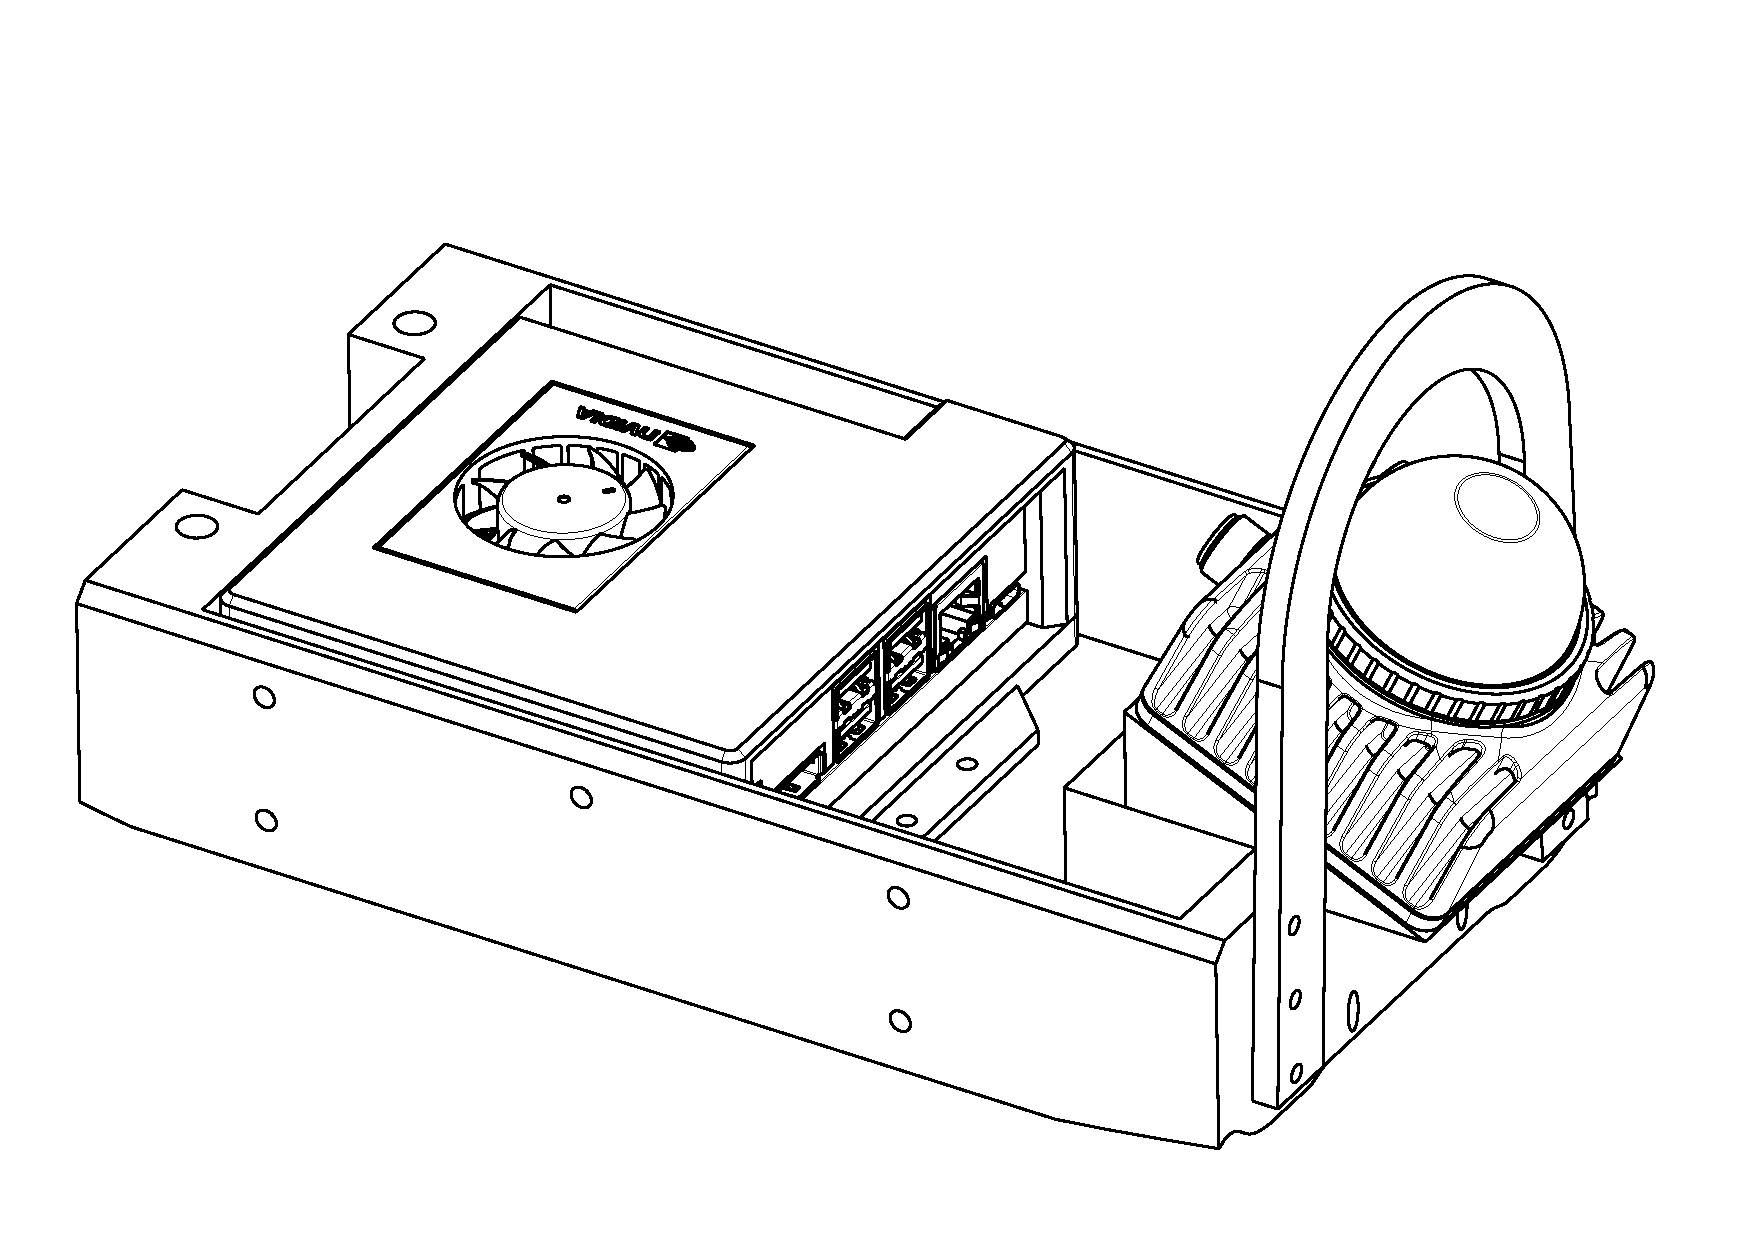
\includegraphics[width=0.6\textwidth]{Images/ComputeBackpack.pdf}
                \caption{Scanned top and CAD model of the compute backpack }
                \label{fig:scanner_and_cad}
            \end{figure}




            \begin{figure}[H]
                \centering
                IMAGE OF COMPUTE BACKPACK
            \end{figure}


            
            \subsubsection{Comminucation with the quadruped}

            % explain how we use webRTC to communicate with the robot (explain whatit is and how it works)
            % explain how we could use the cyclondeDDS because we have access to the newly jailbreaked robot
            
        \subsection{Issues encountered}
            
            %Big battery issue, reverse engineering of the battery, jailbreaking of the robot
            As delivered, the robot was not functionnal as the battery was discharged beyond the point of no return. The battery was disassembled and partly reverse engineered to understand the problem. Even though the battery was not repairable, the reverse engineering allowed us to understand the battery's BMS and how it communicated with the robot. In \cite{battery_reverse_engineering}
            it can be seen that I was able to partly reverse engineer the battery communication protocol. This was shared with others from the open source community actively trying to design a replacement motherboard for the robot. 
            
            The battery was then replaced by a new one and the robot was jailbroken to allow for more control over the robot.
            

            \begin{figure}[H]
                \centering
                \subfigure[Disassembled battery]{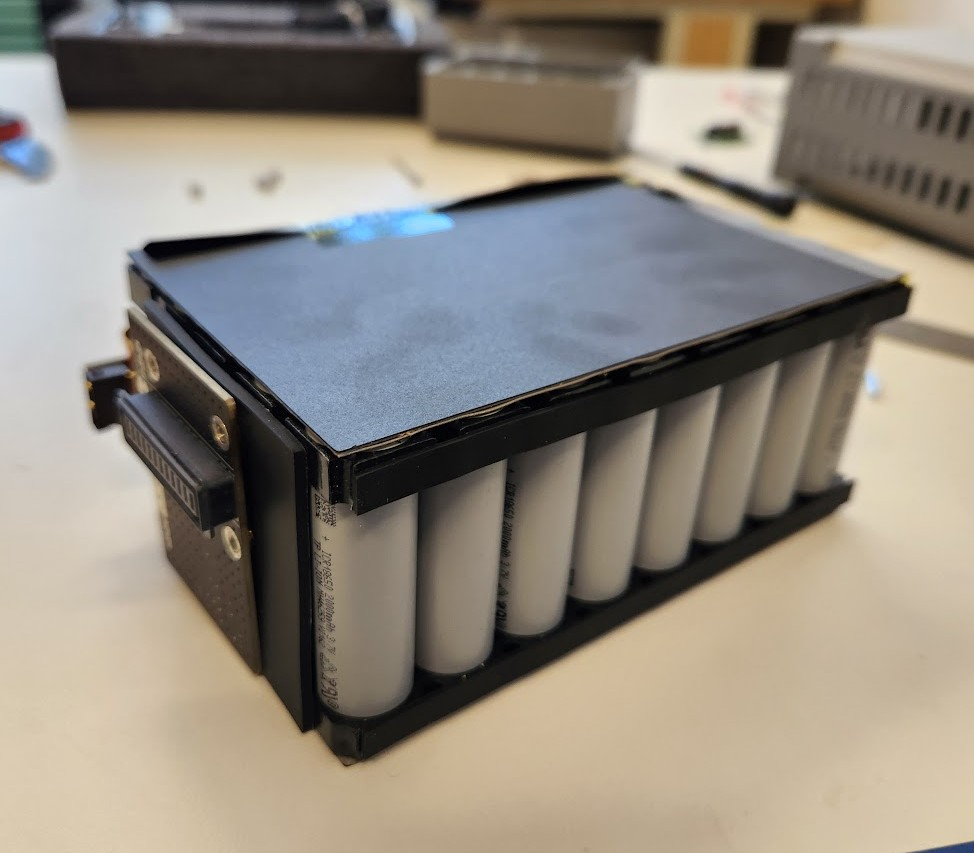
\includegraphics[width=0.4\textwidth]{Images/teardown_battery.jpg}}
                \subfigure[Battery Management System (BMS)]{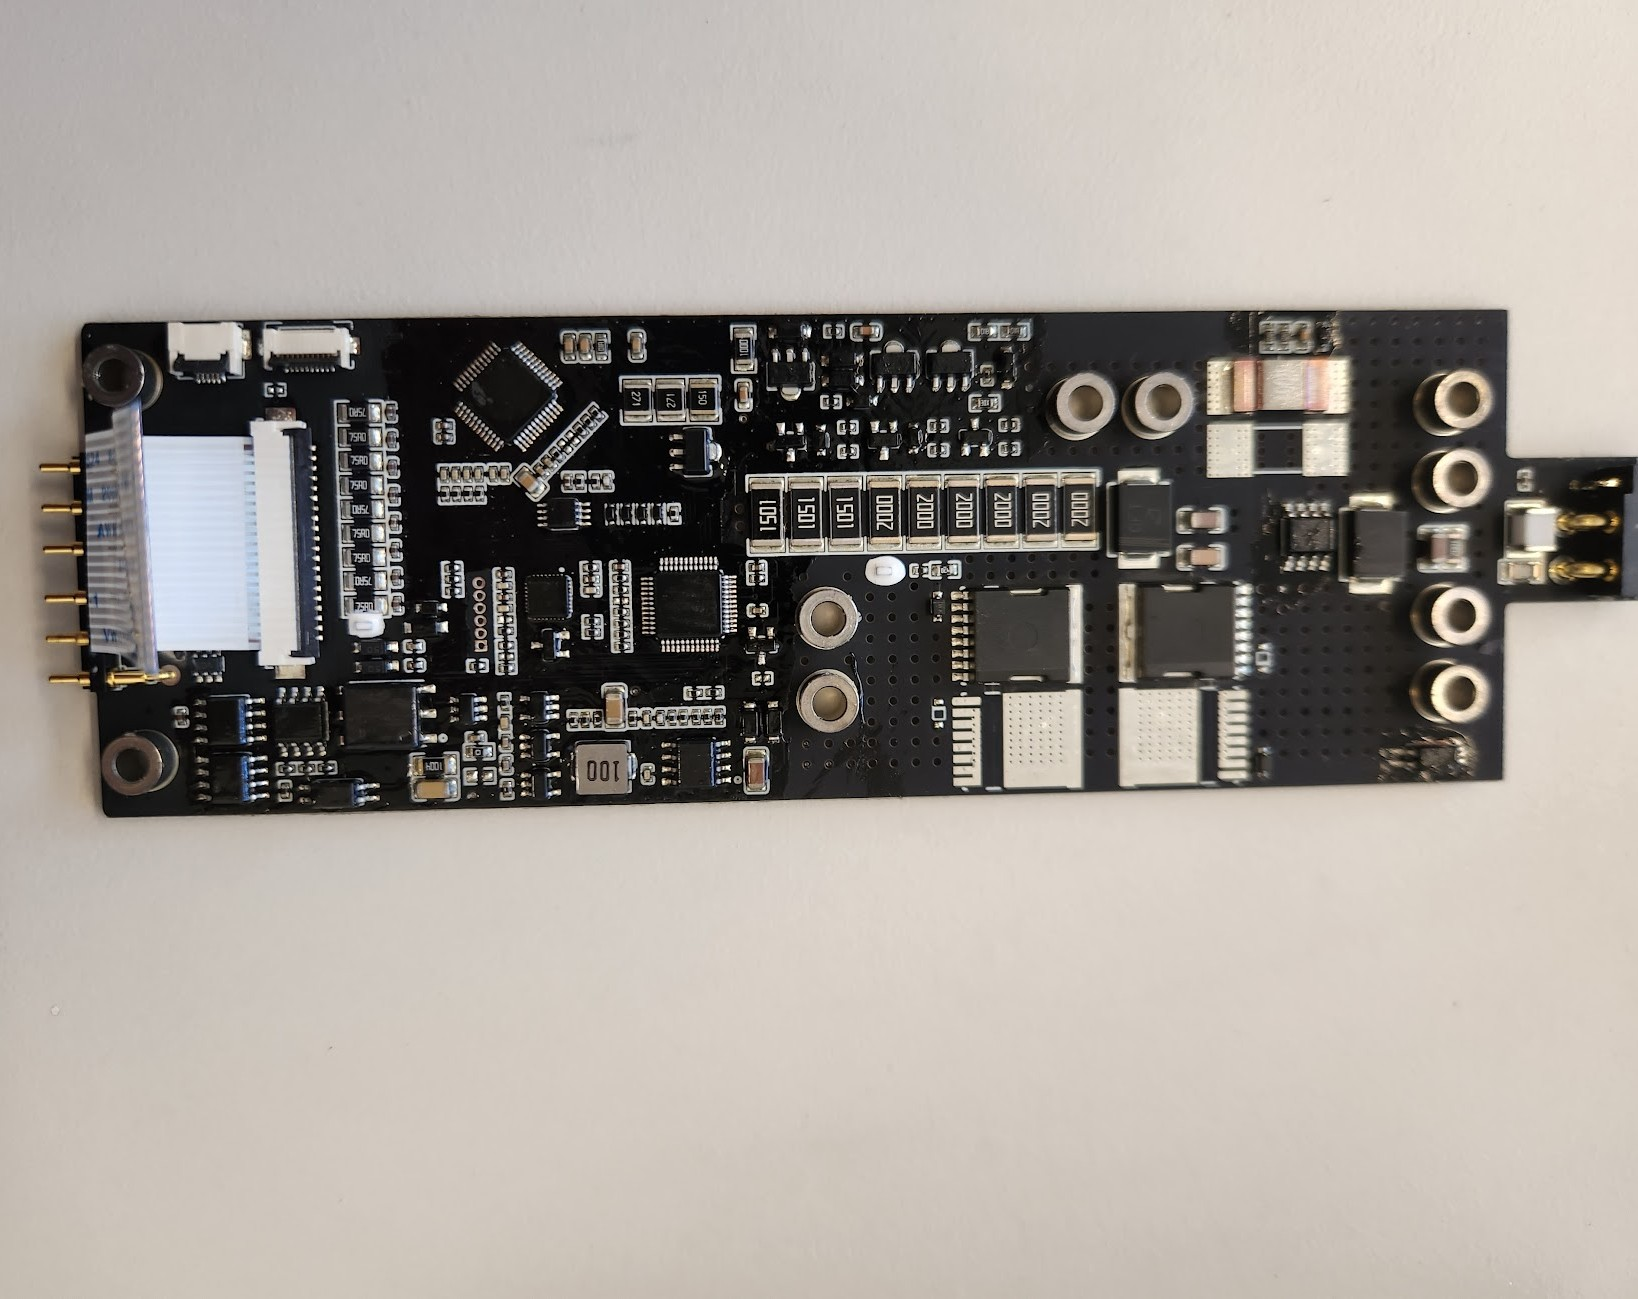
\includegraphics[width=0.44\textwidth]{Images/BMS.jpg}}
                \caption{Disassembled battery and Battery Management System (BMS)}
            \end{figure}


            \begin{figure}[H]
                \centering
                \color{red}LISTING OF THE REVERSE ENGINEERED PROTOCOL OF THE BATTERY
                \caption{Partly reverse engineered battery protocol}
                \label{fig:battery_protocol}
            \end{figure}

            One of the other issues encountered happened after a software update of the robot. We weren't able to connect via SSH to the linux computer inside the robot. This required many days of reverse engineering of the new firmware with the help of other people online.

            The update had removed a vulnerable update mechanism that previously allowed us to gain a root shell to the robot. With that shell, we were then able to change the password of the robot and gain access to the robot via SSH. The new firmware had also prevented us from using the ethernet port of the robot to communicate to the robot using the CyclondeDDS which is one of the Data Distribution Services that ROS can use. This functionality of the robot is usually reserved for the educational version of the GO2, but the company doesn't offer any upgrade from the standard version to the educational version.

            As such, I helped the open source community to design a new unlocking method. For reference, in the previous version, only a version number in a single file needed to be changed from a 2 to a 4 ti unlock every functionality of the robot. The new update brought many new chalenges as every binary was not heavely obfuscated and had increased in size by a factor of 10, every file's checksum was now verified by a yet unknown program, no debuger could be attached as every binary checked their parent process, and many other obfuscation techniques were used.

            The anti debuger technique was quickly bypassed as only the name of the parent process was checked against a list of names, \texttt{gdb-server} not being part of this list made it easy to debug the binaries. Every binary also checked for the presence of a \texttt{tracepid} value, which was solved at first with kernel module that hides the presence of the \texttt{tracepid} value. Other threads were also created to continue monitoring those values in the binaries, but patching the \texttt{pthread\_create} instructions to \texttt{MOV X0, \#0} solved that problem.

            Once the location of the checksum check was identified in a binary, the instruction responsible for the comparaison was patched to always return true : the previsou instruction \texttt{BL <compare>} was replaced by \texttt{MOV X0, \#0}.

            Finaly, the version check was bypassed by consolidating two instruction in one, to in terms have room to set the value of the register \texttt{X0} to 4 as can be seen in the table \ref{tab:patched_instructions}.
            

            % Please add the following required packages to your document preamble:
            % \usepackage[table,xcdraw]{xcolor}
            % Beamer presentation requires \usepackage{colortbl} instead of \usepackage[table,xcdraw]{xcolor}
            \begin{table}[]
                \centering
                \mbox{}\clap{
                \begin{tabular}{|l|l|l|l|l|}
                \hline
                \textbf{Address} & \textbf{Original value} & \textbf{Original Instruction}      & \textbf{Patched value} & \textbf{Patched instruction}       \\ \hline
                \texttt{565BD80} & \texttt{E0 7B BF A9}   & \texttt{stp     x0, x30, {[}sp,\#-0x10{]}!} & \texttt{80 00 80 D2}            & \texttt{mov x0, \#4}                    \\ \hline
                                 & \texttt{63 4D 00 94}   & \texttt{bl      sub\_566F310              } & \texttt{E0 7B BF A9}            & \texttt{stp x0, x30, {[}sp,\#-0x10{]}!} \\ \hline
                                 & \texttt{84 00 00 18}   & \texttt{ldr     w4, \#0x565BD98           } & \texttt{63 4D 00 94}            & \texttt{bl sub\_566F310}                \\ \hline
                                 & \texttt{84 7C 40 93}   & \texttt{sxtw    x4, w4                    } & \texttt{64 00 00 98}            & \texttt{ldrsw X4, \#0x565BD98}          \\ \hline
                \end{tabular}
                }
                \label{tab:patched_instructions}    
                \caption{Patched instructions for version check}
            \end{table}




        \newpage

    \section{Mapping, planning, and exploration algorithms}

        There are three main components to the software architecture of the multi-agent system: mapping, planning, and exploration. Mapping first involves knowing where the robot is and how it is moving, or it's odometry. Planning is often divided in two scales, a local one where we consider what movements the robot is capable of doing, a global one that aims to find the best path to a goal. Exploration uses the two former process as to determine where the robot should go to maximize the information gathered.

        \subsection{Mapping}
            
            \subsubsection{Introduction to SLAM}
            \subsubsection{Comparison of odometry algorithms}
            \subsubsection{LIDAR inertial odometry}
            \subsubsection{Terrain analysis}
            % explain the two terrain analysis we do on the acquired point cloud
        \subsection{Planning}
            \subsubsection{Path planning}
            \subsubsection{2D path planning}
            % Using nav2 as a base and how we convert from a 3D point cloud to a 2D one 
            \subsubsection{Comparison of 3D planning algorithms}

        \subsection{Exploration}
            \subsubsection{Metrics for exploration}
            % show how we calculate the exploration rate using the tools provided in the TARE planner
            % explain the need for a pre-recorded pointcloud of the area we wish to explore
            \subsubsection{TARE-PLANNER}
            % go in details about the process that the TARE-planner uses to explore and the motivations for the original creation of this planner (darpa sub teranean chaleneg)
            \subsubsection{MTARE-PLANNER}
            % multi agent exploration
            \subsubsection{Comparison of exploration algorithms}
            % metion the other exploration planners that are mentioned in the literature and how they compare to TARE and MTARE


    \newpage
    \section{Simulation}
        \subsection{Choosing a simulation environment}

            To test the algorithms and the coordination of the different platforms, a simulation environment was needed. The choice of the simulation environment was based on the following criteria : being able to simulate multiple platforms, being able to simulate the sensors we had on the physical platforms, and the portability of the simulation environment.


            \subsubsection{Gazebo}
                Gazebo is a well known simulation environment in the robotics community. It is widely used and has a large community. It is open source and has a lot of plugins available, for simulation sensors, motion platforms and more. As I was already familiar with it, I first looked at it to build a crude simulation of the 6 wheeled platform. Thanks to the use of ROS2 and ROS2-control for the drive train, I was able to quickly build a simulation of the platform. 

                I was also able to find a working simulation of the Livox Mid-360 LIDAR sensor we chose for every platform. The package \cite{livox_lidar_simulation_fork} was a fork of the original simulation package from Livox \cite{livox_laser_simulation} and was modified to work with the specific LIDAR we are using. 
            \subsubsection{Nvidia Isaac Sim}

                Isaac sim is a high fidelity simulation environment developed by Nvidia. This simulation environment uses a PhysX based physics engine and is able to simulate multiple platforms at once. It is also able to simulate sensors like cameras, LIDARs and IMUs. The main advantage of Isaac sim is it's high fidelity and parallelization. However, this also brings a lot of complexity and the need for a RTX GPU to run it.

                The high overhead, complexity, low portability and the fact that it was not open source made me choose Gazebo over Isaac sim for the simulation of the platforms.

                In addition, the LIDAR we are using has a non repetitive pattern, which is not currently supported by Isaac sim and would have required a lot of work to simulate.

                I did experiment with Isaac sim to simulate the quadruped platform, as it was the most complex platform to simulate and there existed a simulation of the robot in Isaac sim.
        \subsection{Simulating sensors}
            \subsubsection{LIDAR}

            \begin{figure}[H]
                \centering
                \subfigure[Gazebo simulation environment]{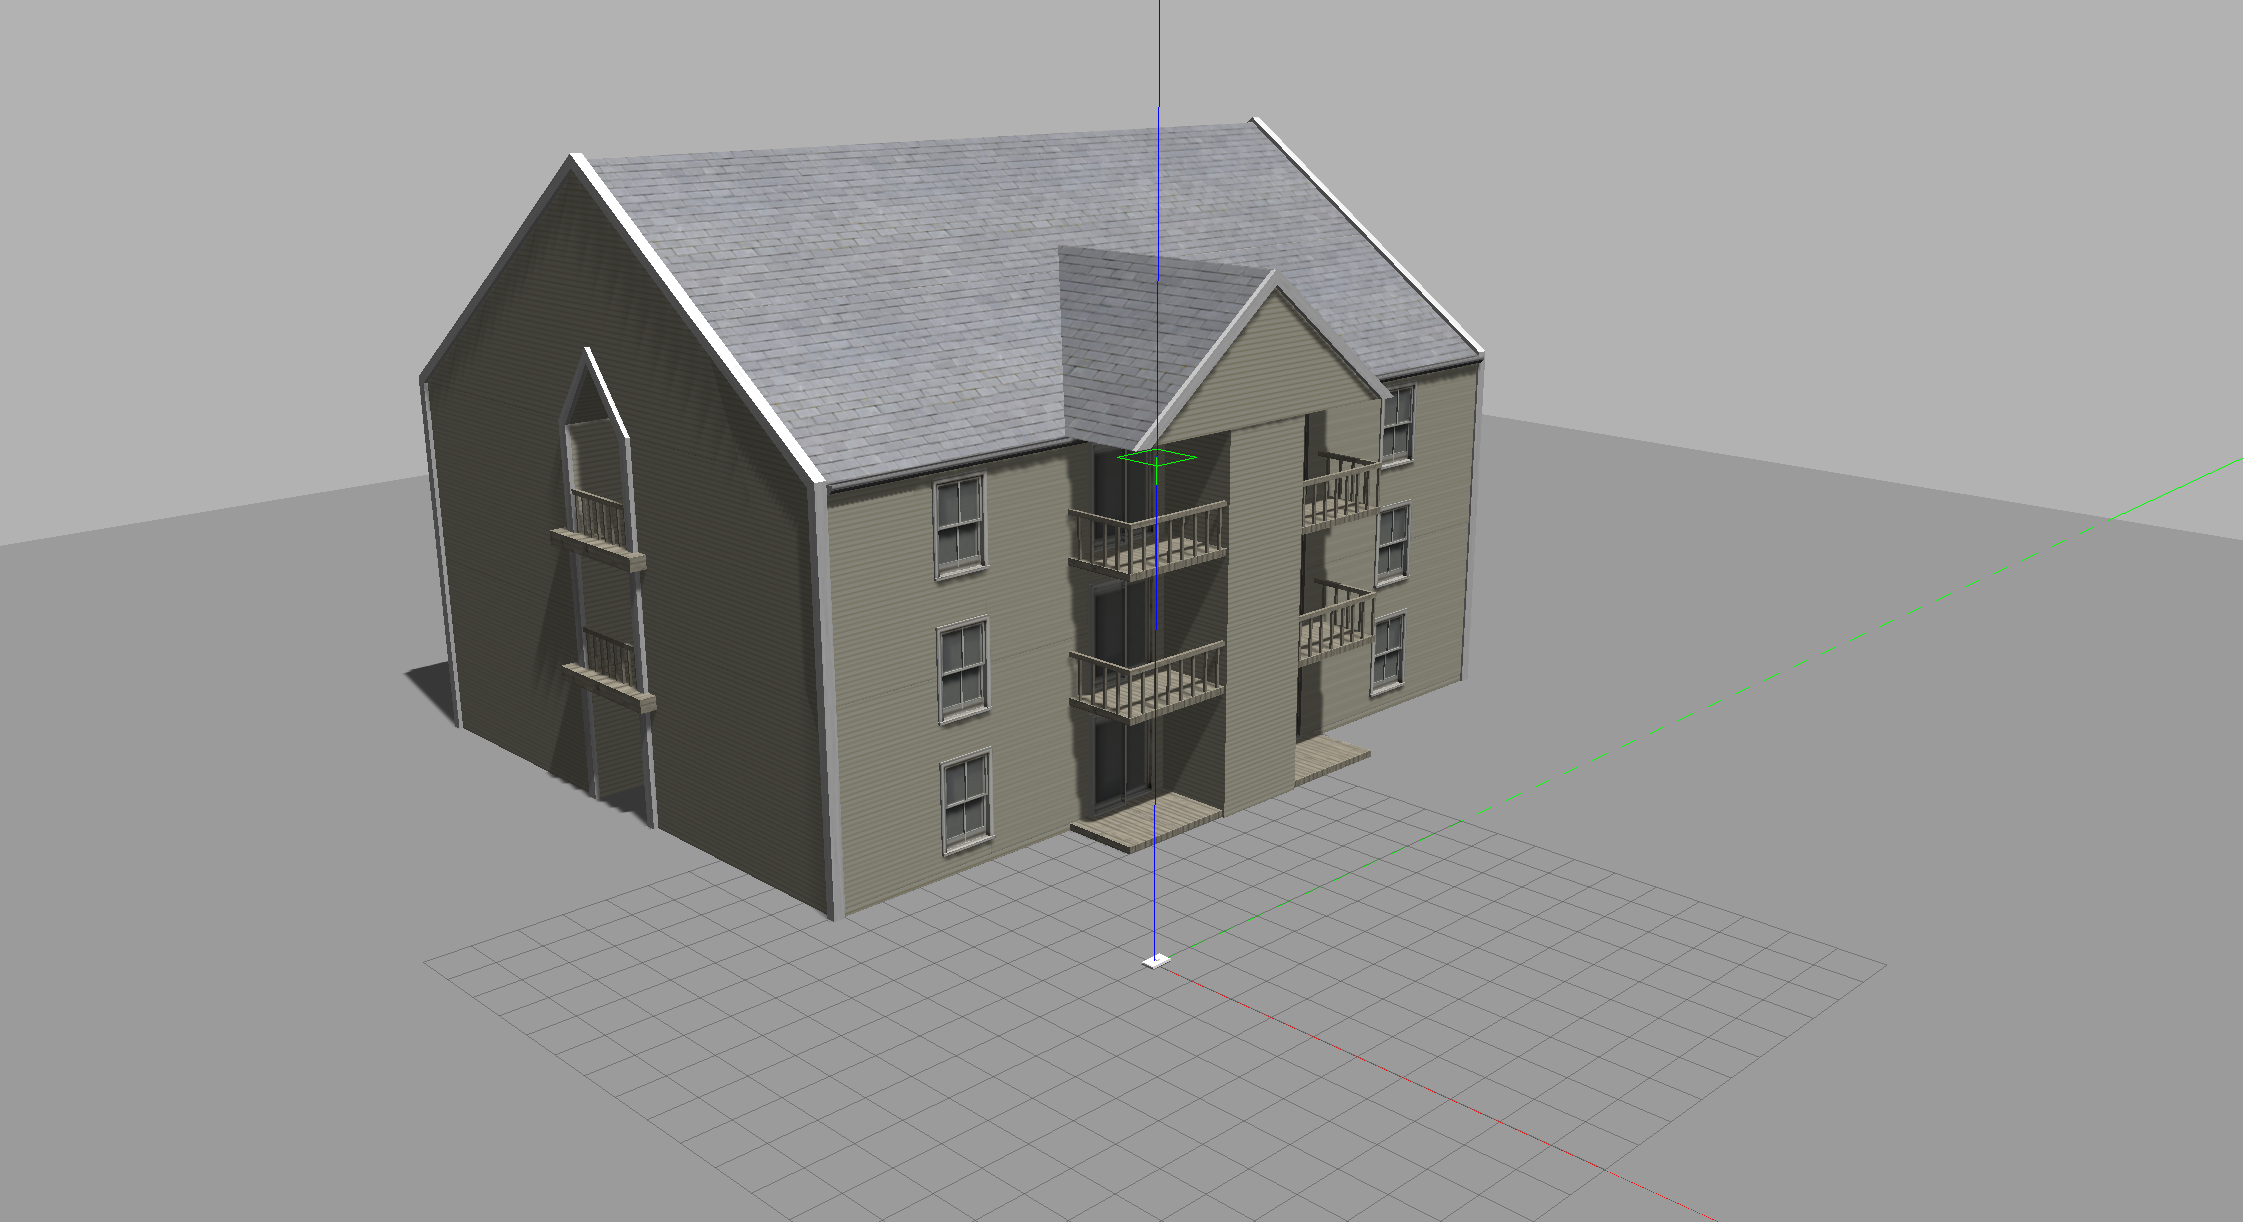
\includegraphics[height=0.25\textwidth]{Images/croped lidar simulation gazebo.png}}
                \subfigure[Point cloud from simulated LIDAR]{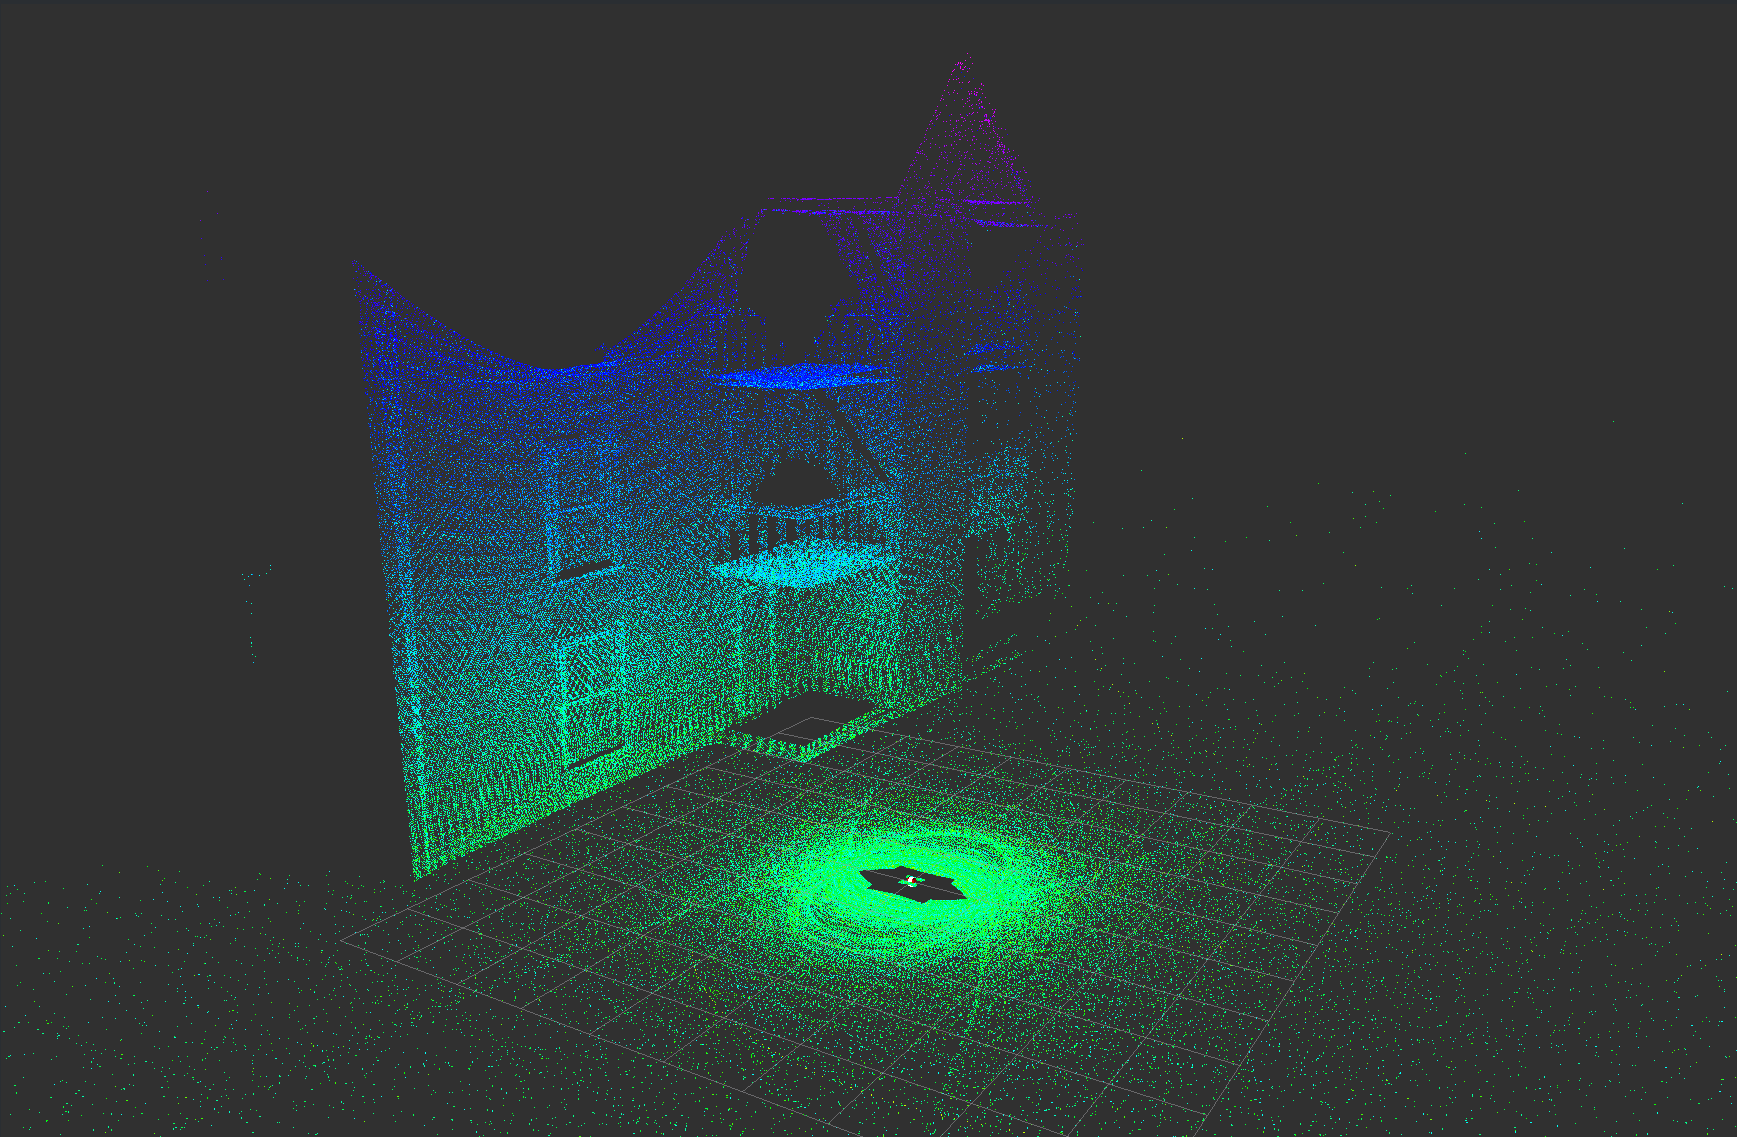
\includegraphics[height=0.25\textwidth]{Images/croped lidar simulation rviz2.png}}
                \caption{Simulated LIDAR in Gazebo and point cloud in RVIZ2}
            \end{figure}

            \subsubsection{IMU}
            \subsubsection{Camera}
        \subsubsection{Simulated world}

        As the target application of this multi agent exploration is to map a construction environment, a simulated world of an office in construction was created. The world is mainly based on the Gazebo office world by Clearpath Robotics and has two versions : one in construction with wall being build and construction equipement all over, and one where the office is constructed as can be seen in figure \ref{fig:office_world}.

        \begin{figure}
            \centering
            \color{red} INSERT PICTURE OF THE OFFICE WORLD IN CONSTRUCTION AND CONSTRUCTED
            %\subfigure[Office in construction]{\includegraphics[width=0.45\textwidth]{Images/office_world.png}}
            %\subfigure[Office constructed]{\includegraphics[width=0.45\textwidth]{Images/office_world_constructed.png}}
            \caption{Office world in construction and constructed}
            \label{fig:office_world}
        \end{figure}


    \section{Conclusion}
    %\addcontentsline{toc}{section}{Conclusion}

        Conclusion     

    \newpage
    \bibliography{refs} % Entries are in the refs.bib file
    \addcontentsline{toc}{section}{Bibliography}

    \newpage
    \addcontentsline{toc}{section}{Glossaire}
    \printnoidxglossaries %glossaire, dans le fichier lexique.tex

    \newpage
    \addcontentsline{toc}{section}{List of figures}
    \listoffigures


    \newpage
    \section*{Annexe}
    \addcontentsline{toc}{section}{Annexe}
    Uncomment input annexe when needed
    %\begin{lstlisting}[style=yaml, caption={TARE planner parameter configuration for Unitree GO2}, label={lst:tare_config}]
tare_planner_node:
  ros__parameters:
    sub_start_exploration_topic_ : /start_exploration
    sub_terrain_map_topic_ : /terrain_map
    sub_terrain_map_ext_topic_ : /terrain_map_ext
    sub_state_estimation_topic_ : /state_estimation_at_scan
    sub_registered_scan_topic_ : /registered_scan
    sub_coverage_boundary_topic_ : /sensor_coverage_planner/coverage_boundary
    sub_viewpoint_boundary_topic_ : /navigation_boundary
    sub_nogo_boundary_topic_ : /sensor_coverage_planner/nogo_boundary
    sub_joystick_topic_ : /joy
    sub_reset_waypoint_topic_ : /reset_waypoint
    pub_exploration_finish_topic_ : exploration_finish
    pub_runtime_breakdown_topic_ : runtime_breakdown
    pub_runtime_topic_ : /runtime
    pub_waypoint_topic_ : /way_point
    pub_momentum_activation_count_topic_ : momentum_activation_count

    kAutoStart : true
    kRushHome : true
    kUseTerrainHeight : true
    kCheckTerrainCollision : true
    kExtendWayPoint : false
    kUseLineOfSightLookAheadPoint : false
    kNoExplorationReturnHome : false
    kExtendWayPointDistanceBig : 1.0
    kExtendWayPointDistanceSmall : 0.5  
    kKeyposeCloudDwzFilterLeafSize : 0.2
    kRushHomeDist : 0.05 # 5.0
    kAtHomeDistThreshold : 0.75 # 0.5
    kTerrainCollisionThreshold : 0.5
    kLookAheadDistance : 8.0
    kUseMomentum : false 
    kDirectionChangeCounterThr : 6
    kDirectionNoChangeCounterThr : 5
    kResetWaypointJoystickAxesID : 2

    # PlanningEnv
    kUseFrontier : true
    kFrontierClusterTolerance : 2.0 # 1.0
    kFrontierClusterMinSize : 5 #10
    kUseCoverageBoundaryOnFrontier : false
    kUseCoverageBoundaryOnObjectSurface : false

    # Rolling occupancy grid
    rolling_occupancy_grid/resolution_x : 0.2
    rolling_occupancy_grid/resolution_y : 0.2
    rolling_occupancy_grid/resolution_z : 0.2

    kSurfaceCloudDwzLeafSize : 0.3 # 0.3
    kCollisionCloudDwzLeafSize : 0.2 # 0.2
    kKeyposeCloudStackNum : 5 # 5
    kPointCloudRowNum : 20 # 50
    kPointCloudColNum : 20 # 50
    kPointCloudLevelNum : 30
    kMaxCellPointNum : 100000 # 100000
    kPointCloudCellSize : 5.0 # 18.0
    kPointCloudCellHeight : 1.8 # 1.8
    kPointCloudManagerNeighborCellNum : 5 # 5
    kCoverCloudZSqueezeRatio : 2.0 # 2.0

    # KeyposeGraph
    keypose_graph/kAddNodeMinDist : 1.0
    keypose_graph/kAddNonKeyposeNodeMinDist : 0.5
    keypose_graph/kAddEdgeConnectDistThr : 3.0
    keypose_graph/kAddEdgeToLastKeyposeDistThr : 3.0
    keypose_graph/kAddEdgeVerticalThreshold : 1.0
    keypose_graph/kAddEdgeCollisionCheckResolution : 0.4
    keypose_graph/kAddEdgeCollisionCheckRadius : 0.4
    keypose_graph/kAddEdgeCollisionCheckPointNumThr : 1

    # ViewPointManager
    viewpoint_manager/number_x : 30 # 50
    viewpoint_manager/number_y : 30 # 50
    viewpoint_manager/number_z : 1
    viewpoint_manager/resolution_x : 0.2 # 0.4
    viewpoint_manager/resolution_y : 0.2 # 0.4
    viewpoint_manager/resolution_z : 0.0
    kConnectivityHeightDiffThr : 0.25
    kGreedyViewPointSampleRange : 3 # 3
    kLocalPathOptimizationItrMax : 10 # 10
    kViewPointCollisionMargin : 0.25  # 0.6
    kViewPointCollisionMarginZPlus : 0.5
    kViewPointCollisionMarginZMinus : 0.5
    kCollisionGridZScale : 1.0
    kCollisionGridResolutionX : 0.2
    kCollisionGridResolutionY : 0.2
    kCollisionGridResolutionZ : 0.0
    kCollisionPointThr : 1
    kLineOfSightStopAtNearestObstacle : true
    kViewPointHeightFromTerrain : 0.3  # 0.75
    kViewPointHeightFromTerrainChangeThreshold : 0.2  # 0.6
    kCheckDynamicObstacleCollision : false
    kCollisionFrameCountMax : 3

    kSensorRange : 8.5  # 3.5
    kNeighborRange : 1.5 # 3.0
    kCoverageOcclusionThr : 0.1
    kCoverageDilationRadius : 0.9

    # Grid World
    kGridWorldXNum : 50 # 121
    kGridWorldYNum : 50 # 121
    kGridWorldZNum : 50 # 121
    kGridWorldCellHeight : 3.0 # 3.0
    kGridWorldNearbyGridNum : 5 # 5
    kMinAddPointNumSmall : 1 # 30
    kMinAddPointNumBig : 1 #60
    kMinAddFrontierPointNum : 1 #20
    kCellExploringToCoveredThr : 1
    kCellCoveredToExploringThr: 10 # 10
    kCellExploringToAlmostCoveredThr: 10 # 10
    kCellAlmostCoveredToExploringThr: 20 # 20
    kCellUnknownToExploringThr: 1

    # Visualization (parameters not working I think)
    kExploringSubspaceMarkerColorGradientAlpha : true
    kExploringSubspaceMarkerColorMaxAlpha : 0.8
    kExploringSubspaceMarkerColorR : 0.0
    kExploringSubspaceMarkerColorG : 1.0
    kExploringSubspaceMarkerColorB : 0.0
    kExploringSubspaceMarkerColorA : 1.0
    kLocalPlanningHorizonMarkerColorR : 0.0
    kLocalPlanningHorizonMarkerColorG : 1.0
    kLocalPlanningHorizonMarkerColorB : 0.0
    kLocalPlanningHorizonMarkerColorA : 1.0
    kLocalPlanningHorizonMarkerWidth : 0.05
    kLocalPlanningHorizonHeight : 3.0

\end{lstlisting}



    
\end{document}